
\documentclass[a4paper,UKenglish,cleveref, autoref, thm-restate]{lipics-v2021}
%This is a template for producing LIPIcs articles. 
%See lipics-v2021-authors-guidelines.pdf for further information.
%for A4 paper format use option "a4paper", for US-letter use option "letterpaper"
%for british hyphenation rules use option "UKenglish", for american hyphenation rules use option "USenglish"
%for section-numbered lemmas etc., use "numberwithinsect"
%for enabling cleveref support, use "cleveref"
%for enabling autoref support, use "autoref"
%for anonymousing the authors (e.g. for double-blind review), add "anonymous"
%for enabling thm-restate support, use "thm-restate"
%for enabling a two-column layout for the author/affilation part (only applicable for > 6 authors), use "authorcolumns"
%for producing a PDF according the PDF/A standard, add "pdfa"

% \usepackage{ltexpprt}
\usepackage{footmisc}
\usepackage{hyperref}

% *** MATH PACKAGES ***
%
\usepackage{amsmath}
\usepackage{nicefrac}
\usepackage{array}
\usepackage{lmodern,amssymb}
\usepackage{float}
\usepackage{graphicx}
\usepackage{caption}
\usepackage{subcaption}
\usepackage{tikz}
\usetikzlibrary{positioning}
\usetikzlibrary{shapes.misc}

\usepackage[utf8]{inputenc}
\usepackage[T1]{fontenc}
% \usepackage[english]{babel}
\usepackage{pgfplots}
\usepackage{algorithm}
\usepackage{algpseudocode}
% \usepackage[capitalize]{cleveref}
\usepackage{mathtools}
\usepackage{booktabs}
\usepackage{cleveref}

%\pdfoutput=1 %uncomment to ensure pdflatex processing (mandatatory e.g. to submit to arXiv)
%\hideLIPIcs  %uncomment to remove references to LIPIcs series (logo, DOI, ...), e.g. when preparing a pre-final version to be uploaded to arXiv or another public repository

%\graphicspath{{./graphics/}}%helpful if your graphic files are in another directory

\bibliographystyle{plainurl}% the mandatory bibstyle

\title{\Large Exact Lower Bounds for the Number of Comparisons in Selection}

%\titlerunning{Dummy short title} %TODO optional, please use if title is longer than one line

% \author{Jane {Open Access}}{Dummy University Computing Laboratory, [optional: Address], Country \and My second affiliation, Country \and \url{http://www.myhomepage.edu} }{johnqpublic@dummyuni.org}{https://orcid.org/0000-0002-1825-0097}{(Optional) author-specific funding acknowledgements}

\author{Josua Dörrer}{University Stuttgart}{}{}{}
\author{Konrad Gendle}{University Stuttgart}{}{}{}
\author{Johanna Hofmann}{University Stuttgart}{}{}{}
\author{Julius von Smercek}{University Stuttgart}{}{}{}
\author{Andreas Steding}{University Stuttgart}{}{}{}
\author{Florian Stober}{University Stuttgart}{}{}{}

%TODO mandatory, please use full name; only 1 author per \author macro; first two parameters are mandatory, other parameters can be empty. Please provide at least the name of the affiliation and the country. The full address is optional. Use additional curly braces to indicate the correct name splitting when the last name consists of multiple name parts.

\author{Joan R. Public\footnote{Optional footnote, e.g. to mark corresponding author}}{Department of Informatics, Dummy College, [optional: Address], Country}{joanrpublic@dummycollege.org}{[orcid]}{[funding]}

\authorrunning{J. Open Access and J.\,R. Public} %TODO mandatory. First: Use abbreviated first/middle names. Second (only in severe cases): Use first author plus 'et al.'

\Copyright{Jane Open Access and Joan R. Public} %TODO mandatory, please use full first names. LIPIcs license is "CC-BY";  http://creativecommons.org/licenses/by/3.0/

\ccsdesc[100]{\textcolor{red}{Replace ccsdesc macro with valid one}} %TODO mandatory: Please choose ACM 2012 classifications from https://dl.acm.org/ccs/ccs_flat.cfm 

\keywords{Dummy keyword} %TODO mandatory; please add comma-separated list of keywords

\category{} %optional, e.g. invited paper

\relatedversion{} %optional, e.g. full version hosted on arXiv, HAL, or other respository/website
%\relatedversiondetails[linktext={opt. text shown instead of the URL}, cite=DBLP:books/mk/GrayR93]{Classification (e.g. Full Version, Extended Version, Previous Version}{URL to related version} %linktext and cite are optional

%\supplement{}%optional, e.g. related research data, source code, ... hosted on a repository like zenodo, figshare, GitHub, ...
%\supplementdetails[linktext={opt. text shown instead of the URL}, cite=DBLP:books/mk/GrayR93, subcategory={Description, Subcategory}, swhid={Software Heritage Identifier}]{General Classification (e.g. Software, Dataset, Model, ...)}{URL to related version} %linktext, cite, and subcategory are optional

%\funding{(Optional) general funding statement \dots}%optional, to capture a funding statement, which applies to all authors. Please enter author specific funding statements as fifth argument of the \author macro.

\acknowledgements{I want to thank \dots}%optional

%\nolinenumbers %uncomment to disable line numbering



%Editor-only macros:: begin (do not touch as author)%%%%%%%%%%%%%%%%%%%%%%%%%%%%%%%%%%
\EventEditors{John Q. Open and Joan R. Access}
\EventNoEds{2}
\EventLongTitle{42nd Conference on Very Important Topics (CVIT 2016)}
\EventShortTitle{CVIT 2016}
\EventAcronym{CVIT}
\EventYear{2016}
\EventDate{December 24--27, 2016}
\EventLocation{Little Whinging, United Kingdom}
\EventLogo{}
\SeriesVolume{42}
\ArticleNo{23}
%%%%%%%%%%%%%%%%%%%%%%%%%%%%%%%%%%%%%%%%%%%%%%%%%%%%%%

% Commands
%! parser=off
\newcommand\smallO{
\mathchoice
{{\scriptstyle\mathcal{O}}}% \displaystyle
{{\scriptstyle\mathcal{O}}}% \textstyle
{{\scriptscriptstyle\mathcal{O}}}% \scriptstyle
{\scalebox{.50}{$\scriptscriptstyle\mathcal{O}$}}%\scriptscriptstyle
}
%! parser=on
\DeclareMathOperator{\N}{\mathbb{N}}
\newcommand{\set}[2]{\left\{\, \mathinner{#1}\vphantom{#2}\: \left|\: \vphantom{#1}\mathinner{#2} \right.\,\right\}}
\newcommand\ie{i.e\@., }
\newcommand{\sse}{\subseteq}
\newcommand{\pchild}[3]{{#1}\kern-1pt{+}{#2}{#3}}
\newcommand{\dual}[1]{{#1}^{\delta}}
\newcommand{\reduced}[1]{\operatorname{red}{#1}}
\newcommand{\less}[2]{D_{#1}(#2)}
\newcommand{\greater}[2]{U_{#1}(#2)}
% \newtheorem{definition}{Definition}[section]
% \newtheorem{observation}{Observation}[section]
% \newtheorem{remark}{Remark}[section]

\newcommand{\projectURL}[0]{https://github.com/JGDoerrer/selection_generator}
\newcommand{\projectServer}[0]{GitHub}

% \newcommand{\projectURL}[0]{https://drive.google.com/file/d/117g3E-0LrnQKdUrKN9jyYhDGjvKM81M1} % todo: final-version
% \newcommand{\projectServer}[0]{Drive} % todo: final-version

\begin{document}

\maketitle
% // ===================================================

\begin{abstract} \small\baselineskip=9pt
  Selection is the problem of finding the $i$-th smallest element among $n$ elements.
  We apply computer search to find optimal algorithms for small instances of the selection problem.
  Using new algorithmic ideas, we established tighter lower bounds for the number of comparisons required, denoted as $V_i(n)$.
  Our results include optimal algorithms for $n$ up to 15 and arbitrary $i$, and for $n=16$ when $i \leq 6$.
  We determined the precise values $V_7(14) = 25$, $V_6(15) = V_7(15) = 26$, and $V_8(15) = 27$, where previously, only a range was known.
%  We computed $V_i(16)$ for $i \leq 6$ and determined a new lower bound for $V_7(16)$ and $V_8(16)$. 

\end{abstract} % newline above is important for formatting

% delete block
\section*{To Do (delete section later)}
\begin{itemize}
  \item Florian: herausstellen was neu ist und was übernommen ist
  \item Florian: when presenting an overview state explicitly that the more details are coming later (3.3.1 \& 6. paragraph of 3.3.3) (6th paragraph of 3.3.3, which also shouldn't be the first place in the paper that you
  mention doing anything other than using nauty).
  \item Julius: Poset Abbildungen kleiner machen -> scale 0.7
  \item Konrad: Isomorphism nur an einer Stelle im Paper beschreiben
  \item Johanna: Table 2 weg; Abbildung minimax weg; Ergebnisstabelle (Tabelle 5 und 6) in Anhang; Kurze Tabelle in Text (nur Median)
  \item Predecessor Section ist zu lang -> kürzer
\end{itemize}
% delete above block

\section{Motivation} \label{sec:motivation}

The problem of selecting the $i$-th smallest element in a list of $n$ elements is a well-known problem in computer science called \textit{selection}.
Explicitly, we concern ourselves with the optimal worst-case selection of a single element from a set of initially unordered unique elements, measuring the cost by the number of comparisons.
We denote this cost as $V_i(n)$.

For selecting the smallest element, optimal algorithms are known with $V_1(n) = n - 1$.
For the second smallest element, it is known that $V_2(n) = n - 2 + \lceil \log n\rceil$~\cite{Knuth1973} (all logarithms are to base $2$).
In general, the selection problem is solvable in linear time using the median of medians algorithm~\cite{Blum1972}.
Looking at the special case of selecting the median $i = \nicefrac{n}{2}$, the best-known algorithm requires $2.95n$ comparisons~\cite{dor1999selecting}.
For other values of $i$, the algorithm in~\cite{dor1999selecting} requires fewer comparisons, thus providing a general upper bound.
This presents a significant gap compared to the best-known lower bound, which is $\left (1 + H(\nicefrac{i}{n}) \right ) \cdot n + \Omega(\sqrt n)$, where $H(x) = x \cdot \log \frac{1}{x} + (1 - x) \log \frac{1}{1 - x}$~\cite{bent1985finding}.
For the median, this lower bound is $2 \cdot n - \smallO(n)$.
Paterson conjectured that the lower bound for selecting the median is $n \log_{4/3} 2 \approx 2.41n$~\cite{paterson1996progress}.
To improve these bounds toward tightness, it is essential to have known optimal reference points that general approaches can be compared against.

Gasarch, Kelly, and Pugh~\cite{Gasarch1996} were the first to use computer search to find optimal selection algorithms for fixed $n$ and $i$.
Oksanen continued this line of work, improving upon the previously known lower bounds~\cite{Oksanen2006}.
His results and the computer program he used to obtain them are available on his website~\cite{Oksanen}, but have not been published in a scientific journal.

We will also tackle the selection problem using computer search.
We reimplement the minimax algorithm used in~\cite{Gasarch1996,Oksanen,Oksanen2006} and improve upon it by introducing suitable heuristics.
Then we explore a different search strategy, the backward search, which is another significant improvement over the minimax algorithm.
A quote from Miguel de Cervantes from Don Quijote will hold true for this article: ``the journey is better than the inn''~\cite{cervantes_don_quijote}.
So buckle up.

\subsection{Contribution.}
In this work, we apply two different search algorithms to finding optimal algorithms for selection.
The first, which we will call forward search in the remainder of this article, is based on the minimax algorithm also used by Gasarch et.\ al\@.~\cite{Gasarch1996} and Oksanen~\cite{Oksanen,Oksanen2006}.
We introduce a novel pruning criterion based on the notion of compatible solutions, and demonstrate that this leads to a significant improvement compared to the benchmark implementation from~\cite{Oksanen}.

The second algorithm, the backward search, is based on an entirely different idea.
Here, the start and endpoint of the search switch places.
This type of search has not been applied to the selection problem before, and its efficient application poses several challenges, the solution of which is the main technical contribution of this work.

One such challenge is the use of reduced posets.
A poset is reduced by removing all elements that cannot be the $i$-th smallest.
In the forward search this is a straightforward optimization to reduce the search space.
To apply this optimization in the backward search, we show that reduced posets are well-behaved, in a way that allows us to efficiently reverse the reduction.

Another challenge, more of an engineering nature, is the need for an efficiently computable normal form.
The goal of the normal form is to identify isomorphic posets and thus reduce the size of the search space.
A normal form can be computed using the well-known \text{nauty} tool~\cite{MCKAY201494}.
However, a call to \texttt{nauty} is expensive compared to the other steps in the backward search.
Thus we spend a lot of effort on being able to avoid a call to \texttt{nauty} in many cases when computing the normal form.

Using our two algorithms, we obtained the following results:
\begin{enumerate}
  \item We confirm most of the values $V_i(n)$ computed by Oksanen and correct an error in his work which states that $V_5(15)$ would be $25$~\cite{Oksanen}.
        We show that the optimal algorithm requires one comparison fewer, that is $V_5(15) = 24$.
  \item We determined the precise values $V_7(14) = 25$, $V_6(15) = V_7(15) = 26$, and $V_8(15) = 27$.
        Previously, only a range of values was known for these instances.
  \item We computed $V_i(16)$ for $i \leq 6$ and determined a better lower bound for $V_7(16)$ and $V_8(16)$.
\end{enumerate}


\section{Fundamentals}

\subsection{Posets.}
A partial order is a reflexive, transitive, and antisymmetric relation.
A partially ordered set, short \emph{poset}, is a set $\Omega$ with a partial order $P \subseteq \Omega \times \Omega$.
By a slight abuse of notation, we denote the poset by $P$ as well.
When necessary, we write $\Omega_P$ to refer to the underlying set.
Throughout this paper, $\Omega$ is finite.
By $E_n$ we denote the unordered poset on $n$ elements, where each element is related only to itself.
Two posets $P$ and $Q$ are \emph{isomorphic} if there is a bijective mapping $\varphi: \Omega_P \to \Omega_Q$ such that $(u, v) \in R \iff (\varphi(u), \varphi(v)) \in Q$ for all $u, v \in \Omega_P$.
The \emph{dual} of a poset $P$ is obtained by reversing the direction of all edges, \ie $\dual{P} = \set{(v,u)}{(u,v) \in P}$.
Given a poset $P$, its \emph{Hasse diagram} $H$ is given by the smallest subset $H \sse \Omega \times \Omega$ such that $P$ is the reflexive, transitive closure of $H$.
We denote by $\pchild{P}{a}{b}$ the transitive closure of $P \cup \{(a, b)\}$.
By $P|_{\Omega'}$ we denote the restriction of $P$ to $\Omega'$.
The downset of an element $a$ is $\less{P}{a} = \set{b \in \Omega_P}{b \le a}$, and the upset is $\greater{P}{a} = \set{b \in \Omega_P}{b \ge a}$.

\subsection{The Selection Problem.}
The selection problem is, given a poset $P$ and an integer $i$, to determine the $i$-th smallest of the $n$ elements in $\Omega_P$ where we already know the relation $P$.
We denote an instance of the \emph{selection problem}, or problem for short, by $(P, i)$.
The notion of isomorphism naturally extends to selection problems.
For the dual, we have $\dual{(P, i)} = (\dual{P}, n - i + 1)$.
The problem $(P, i)$ is \emph{reduced} if each element has at most $i - 1$ smaller elements and at most $n - i$ larger elements.
We denote the reduced problem corresponding to $(P, i)$ by $\reduced{(P, i)}$.
Hence, each element can still be the $i$-th smallest.

\subsection{Selection Algorithms.}
A selection algorithm is a binary decision tree.
Each node is labeled with a selection problem.
The root node is labeled with $(E_n, i)$.
The leaf nodes are labeled with \emph{solved} problems $(P, i)$ that have a unique element $a \in \Omega_P$, such that $|\less{P}{a}| = i$ and $|\greater{P}{a}| = n - i + 1$.
Thus, $a$ is the $i$-th smallest element.

The selection algorithm associates each inner node $(P, i)$ with a comparison $\{a, b\}$, meaning that the algorithm compares $a$ with $b$ as its next step.
The two children, $(\pchild{P}{a}{b}, i)$ and $(\pchild{P}{b}{a}, i)$, correspond to the two possible outcomes of the comparison $a < b$ and $a > b$.
The number of comparisons required by the algorithm (in the worst case) is the maximum length of a path from the root to any leaf.


\subsection{Minimum Number of Comparisons.}

Let $V_i(n)$ denote the minimum number of comparisons required to select the $i$-th smallest out of $n$ elements in the worst case.
We prove the following transfer lemma for lower bounds, showing that if $k$ is a lower bound for selecting the $i$-th smallest from $n$ elements, then selecting the $i$-th smallest from $n + 1$ elements requires at least $k + 1$ comparisons.

\begin{lemma} \label{lemma:previous_next_poset}
  $V_i(n + 1) \geq V_i(n) + 1$.
\end{lemma}

\begin{proof}
  Let $k = V_i(n + 1)$.
  There exists an algorithm that selects the $i$-th smallest from $n + 1$ elements using $k$ comparisons.
  We now construct an algorithm that selects the $i$-th smallest from $n$ elements using at most $k - 1$ comparisons.
  Let $a$ and $b$ be the two elements compared first by the algorithm for $n + 1$ elements.
  Replace $a$ with a new element $\omega$ that is larger than any other element in the input of the algorithm.
  The algorithm still returns the $i$-th smallest of the remaining $n$ elements.
  Any comparison involving $a = \omega$ can be skipped, as $\omega$ is always larger.
  In particular, the first comparison is skipped, reducing the number of comparisons by at least $1$.
  Thus, we obtain an algorithm for selecting the $i$-th smallest from $n$ elements using $k - 1$ comparisons.
\end{proof}

\begin{remark}
  It appears that Oksanen was unaware of \Cref{lemma:previous_next_poset}, as the ranges provided in his table could be improved using this Lemma~\cite{Oksanen}.
\end{remark}

Note that the bound in \Cref{lemma:previous_next_poset} is tight for some instances, as can be seen from $V_1(n) = n - 1$.
An easy corollary to the lemma is $V_{i + 1}(n + 1) \geq V_i(n) + 1$, which follows immediately from the next lemma.

Let $V_i(P)$ denote the minimum number of comparisons required to select the $i$-th smallest element of the poset $P$ in the worst-case.
$V_i(n)$ is the special case $V_i(E_n)$.
We prove the following lemma showing that the cost of selection remains unchanged when considering the dual problem.

\begin{lemma} \label{lemma:dual_poset_allowed}
  $V_i(P) = V_{n - i + 1}(\dual{P})$
\end{lemma}

\begin{proof}
  Given $V_i(P)$, we know there exists an algorithm that determines the $i$-th smallest element in $P$ using exactly that many comparisons.
  By viewing this algorithm as a binary decision tree and swapping all the children, we obtain an algorithm for selecting the $i$-th largest element in $\dual{P}$, which is also the $(n - i + 1)$-th smallest element of $\dual{P}$.
\end{proof}

\section{Methods and Tools}

In this section, we describe our two main approaches to determining $V_i(n)$: the forward search and the backward search.
The forward search follows the approach used by Oksanen~\cite{Oksanen2006}.
We enhance it by using a pruning technique based on compatible solutions.
The backward search is a novel approach that has not been previously applied to the problem of selection.
It allows us to further improve the computation of optimal selection algorithms.% todo: improve how

\subsection{Data Structures and Isomorphism Testing.}
The key to reducing the search space is to consider only reduced problems and detect isomorphic problems.
Isomorphism testing is performed by computing a \emph{canonical} representative.
For the backward search, we use a custom algorithm to compute a canonical representative.
For complicated cases, our custom algorithm uses \texttt{nauty}~\cite{MCKAY201494} as a fallback.
For the forward search, we use a best-effort approximation to reduce the cost of computing the representative, at the expense of a slightly larger search space.

By \Cref{lemma:dual_poset_allowed}, we do not need to distinguish a problem from its dual.
We take advantage of this by switching to the dual if $i \leq \frac{n+1}{2}$.
If $i = \frac{n+1}{2}$, one of the two is chosen deterministically.
This is described in more detail in \Cref{sec:backward:normal_form}.
A \emph{normal} representative is a uniquely reduced representative of the isomorphism class of the problem and its dual.

We store posets as adjacency matrices.
We choose a canonical representative in each isomorphism class so that we have a lower triangular matrix that can be stored using $\frac{n^2 - n}{2}$ bits.

% TODO: hier alle Sachen zu Isomorphism schreiben

% 2 Unterpunkte jeweils Vor- und Rückwärtssuche

\subsection{Forward Search.} \label{chapter:forward_search}
The forward search algorithm is based on the work of Oksanen~\cite{Oksanen2006} and Gasarch et.\ al\@.~\cite{Gasarch1996}.
We first describe the basic algorithm and then discuss the optimizations and pruning techniques we applied.
Our main contribution to the forward search is the introduction of a novel pruning criterion based on compatible solutions.

The forward search starts with the problem $(E_n, i)$ and recursively determines the cost of selecting the $i$-th smallest element of a poset $P$.
Between the two possible outcomes of a comparison, we assume the worst.
However, since the algorithm is free to choose which elements to compare, we seek the comparison with the lowest cost in the worst-case outcome.
Thus, the cost $V_i(P)$ can be expressed as follows:
\begin{equation}
  V_i(P) = \min_{a,b \in \Omega_P} \max \left\{ \,V_i(\pchild{P}{a}{b}),\, V_i(\pchild{P}{b}{a})\,\right\}\,\text{.}
\end{equation}

The algorithms generated by the search program are built by saving, for each problem, the comparison that led to the cheapest result.

To save memory and allow further pruning, we traverse the search tree using a depth-first search approach.
This reduces the maximum number of comparisons assigned to child problems to one less than the best result currently found.
This principle is implemented using a minimax algorithm.

\subsubsection{Compatible Solutions.}
Suppose we have a solved problem $(P, i)$ with a unique $i$-th smallest element $e$.
We then know precisely the set of elements that are smaller than $e$ as well as the set of elements that are larger than $e$.
This observation leads us to the notion of compatible solutions, which is such a partition compatible with the current relation.

\begin{definition}
  The solved problem $(S, i)$ is a \textbf{compatible solution} of the problem $(R, i)$ if $(a, b) \in S \implies (b, a) \notin R$ and $S$ has no relations other than the $n - 1$ relations involving the $i$-th smallest element along with their transitive relations.
\end{definition}

Clearly, a solved problem has exactly one compatible solution.
Let
\begin{equation*}
  \mathcal{C}(P, i) = \{(S, i) \mid (S, i) \text{ is compatible with } (P, i)\}
\end{equation*}
be the set of all solutions compatible with $(P, i)$.
Observe that, given two elements $a,b$ that are unrelated in $P$, every solution compatible with $(P, i)$ is compatible with at least one of $(\pchild{P}{a}{b}, i)$ and $(\pchild{P}{b}{a}, i)$ and thus
\begin{equation}\label{lemma:compatible_union}
\mathcal{C}(P, i) = \mathcal{C}(\pchild{P}{a}{b}, i) \cup \mathcal{C}(\pchild{P}{b}{a}, i)\,\text{.}
\end{equation}

We use the concept of compatible solutions to derive the following lower bound on the number of comparisons required to select the $i$-th smallest element of a poset $P$, which we use as a pruning criterion in the forward search.

\begin{theorem}\label{theorem:compatible_log}
Selecting the $i$-th smallest element of a poset $P$ requires at least $\lceil\log(|\mathcal{C}(P, i)|)\rceil$ comparisons in the worst case.
\end{theorem}

\begin{proof}
  Assume we have an optimal algorithm for selecting the $i$-th smallest element of a poset $P$.
  From \Cref{lemma:compatible_union}, it follows that for every $(S, i)$, there is at least one leaf in the decision tree labeled with $\{(S, i)\}$.
  Hence, there are at least $|\mathcal{C}(P, i)|$ leaves, implying that the height of the tree is at least $\lceil\log(|\mathcal{C}(P, i)|)\rceil$.
\end{proof}

\subsubsection{Optimizations.}

\subparagraph{Caching.}
We can significantly speed up the exploration by caching previous results, even with a simple usage-based ejection policy.
Since the search always imposes an upper bound on the number of comparisons, this also includes unsolved posets, for which we record the currently known minimum.

\subparagraph{Isomorphism Testing.}
In the cache, we store an approximated canonical representative of a problem and its dual, allowing us to detect isomorphic problems.
Preliminary tests showed that the performance gained by computing an approximated normal form, where some isomorphic problems may have different representatives, outweighs the cost induced by the larger search space.

\subparagraph{Maximum Depth.}
We use the minimax search algorithm to cut off unpromising branches.
While searching the possible comparisons of a poset, we keep track of the current best result.
The remaining comparisons are searched with a limited depth, ensuring that only solutions improving the current best result are found.
At the start of a search, possible comparisons are sorted using a heuristic so that the most promising comparisons are searched for first.

\subparagraph{Free Comparison.}
Another pruning criterion, which has already been used in~\cite{Oksanen}, aims to reduce the size of the searched subtree by adding a `useful' comparison to eliminate elements faster.
Explicitly, it searches for unordered elements $u$ and $v$ such that $u$ has at least two elements less than it and no elements greater than it and $v$ has at least two elements greater than it and no elements smaller than it, and adds $u < v$ to the poset.
The new problem is then searched for a solution using the forward search described above without reducing the number of allowed comparisons.
If the new problem is not solvable, then the original problem cannot be solvable either.
This is valid because adding a comparison `for free' does not make the problem harder to solve.
Connecting a small element to a large element can result in many elements being larger or smaller than $i$ elements.
This allows for more elements to be discarded when reducing the poset.

\subsection{Backward Search.} \label{sec:backward}
The backward search is a different kind of search algorithm, which has not been applied to the selection problem before.
The idea is to start with the set of solved problems, and iteratively remove comparisons until the unordered poset is found.
Recently, this approach has been applied with great success to the related problem of determining the exact lower bound for sorting~\cite{stober2022lower}.

\subsubsection{Algorithm.} \label{sec:backward:algorithm}
In this section, we briefly describe the core principles of the backward search algorithm.
The input parameters for the backward search are denoted by $n$ and $i$, similar to the forward search.
A first challenge when starting the search with the set of solved selection problems is that, even if we restrict ourselves to a fixed cardinality $n$ and rank $i$, the set of solved problems remains large.
We overcome this by only enumerating reduced problems.
With this restriction, the starting point of the backward search is $(E_1, 1)$.
%The backward search starts with the solved problem $(E_1, 1)$ and iteratively computes all posets solvable using $k = 1, 2, 3, \dots$ comparisons until the unordered poset $(E_n, i)$ is encountered.
By $A_k$ we denote the set of all reduced selection problems solvable using $k$ comparisons.
For all $n$ and $i$, we have $A_0 = \{(E_1, 1)\}$.
The backward search begins with $A_0$ and iteratively computes, for each problem in $A_k$, the corresponding predecessors, which form the set $A_{k + 1}$.
If $(E_n, i) \in A_\ell$, then $V_i(n) = \ell$.
\Cref{fig:backward-search-tree} illustrates the backward search for $n = 4$ and $i = 2$.

\begin{figure}[t]
  \centering
  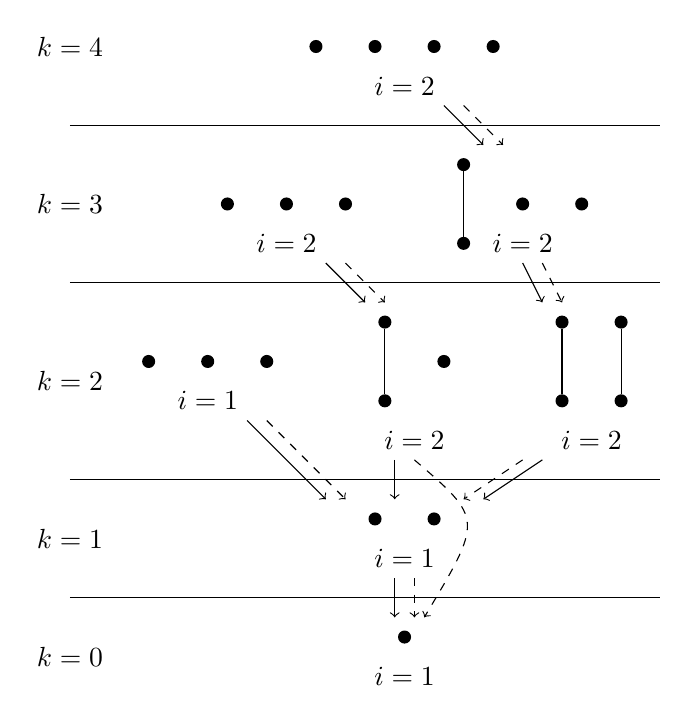
\begin{tikzpicture}

  % Level k = 4
  \node at (-1, 8) {$k=4$};

  \node[circle,fill=black,scale=0.5] (k4_1) at (2.125 + 0 * 0.75, 8) {};
  \node[circle,fill=black,scale=0.5] (k4_2) at (2.125 + 1 * 0.75, 8) {};
  \node[circle,fill=black,scale=0.5] (k4_3) at (2.125 + 2 * 0.75, 8) {};
  \node[circle,fill=black,scale=0.5] (k4_4) at (2.125 + 3 * 0.75, 8) {};
  \node at (2.125 + 0.75 * 1.5, 7.5) {$i=2$};

  \draw[->, dashed] (4, 7.25) -- (4.5, 6.75);
  \draw[->] (3.75, 7.25) -- (4.25, 6.75);

  \draw (-1, 7) -- (6.5, 7);

  % Level k = 3
  \node at (-1, 6) {$k=3$};

  \node[circle,fill=black,scale=0.5] (k3_1) at (1 + 0 * 0.75, 6) {};
  \node[circle,fill=black,scale=0.5] (k3_2) at (1 + 1 * 0.75, 6) {};
  \node[circle,fill=black,scale=0.5] (k3_3) at (1 + 2 * 0.75, 6) {};
  \node at (1 + 0.75, 5.5) {$i=2$};

  \draw[->, dashed] (2.5, 5.25) -- (3, 4.75);
  \draw[->] (2.25, 5.25) -- (2.75, 4.75);

  \node[circle,fill=black,scale=0.5] (k3_4) at (4 + 0 * 0.75, 6.5) {};
  \node[circle,fill=black,scale=0.5] (k3_5) at (4 + 0 * 0.75, 5.5) {};
  \node[circle,fill=black,scale=0.5] (k3_6) at (4 + 1 * 0.75, 6) {};
  \node[circle,fill=black,scale=0.5] (k3_7) at (4 + 2 * 0.75, 6) {};
  \draw (k3_4) -- (k3_5);
  \node at (4 + 0.75, 5.5) {$i=2$};

  \draw[->, dashed] (5, 5.25) -- (5.25, 4.75);
  \draw[->] (4.75, 5.25) -- (5, 4.75);

  \draw (-1, 5) -- (6.5, 5);

  % Level k = 2
  \node at (-1, 3.75) {$k=2$};

  \node[circle,fill=black,scale=0.5] (k2_1) at (0 + 0 * 0.75, 4) {};
  \node[circle,fill=black,scale=0.5] (k2_2) at (0 + 1 * 0.75, 4) {};
  \node[circle,fill=black,scale=0.5] (k2_3) at (0 + 2 * 0.75, 4) {};
  \node at (0 + 0.75, 3.5) {$i=1$};

  \draw[->, dashed] (1.5, 3.25) -- (2.5, 2.25);
  \draw[->] (1.25, 3.25) -- (2.25, 2.25);

  \node[circle,fill=black,scale=0.5] (k2_4) at (3 + 0 * 0.75, 3.5) {};
  \node[circle,fill=black,scale=0.5] (k2_5) at (3 + 0 * 0.75, 4.5) {};
  \node[circle,fill=black,scale=0.5] (k2_6) at (3 + 1 * 0.75, 4) {};
  \draw (k2_4) -- (k2_5);
  \node at (3 + 0.75 * 0.5, 3) {$i=2$};

  \draw[->, dashed] (3.375, 2.75) .. controls (4.25, 2) .. (3.5, 0.75);
  \draw[->] (3.125, 2.75) -- (3.125, 2.25);

  \node[circle,fill=black,scale=0.5] (k2_7) at (5.25 + 0 * 0.75, 3.5) {};
  \node[circle,fill=black,scale=0.5] (k2_8) at (5.25 + 0 * 0.75, 4.5) {};
  \node[circle,fill=black,scale=0.5] (k2_9) at (5.25 + 1 * 0.75, 3.5) {};
  \node[circle,fill=black,scale=0.5] (k2_10) at (5.25 + 1 * 0.75, 4.5) {};
  \draw (k2_7) -- (k2_8);
  \draw (k2_9) -- (k2_10);
  \node at (5.25 + 0.75 * 0.5, 3) {$i=2$};

  \draw[->, dashed] (4.75, 2.75) -- (4, 2.25);
  \draw[->] (5, 2.75) -- (4.25, 2.25);

  \draw (-1, 2.5) -- (6.5, 2.5);

  % Level k = 1
  \node at (-1, 1.75) {$k=1$};

  \node[circle,fill=black,scale=0.5] (k1_1) at (2.875 + 0 * 0.75, 2) {};
  \node[circle,fill=black,scale=0.5] (k1_2) at (2.875 + 1 * 0.75, 2) {};
  \node at (2.875 + 0.75 * 0.5, 1.5) {$i=1$};

  \draw[->, dashed] (3.375, 1.25) -- (3.375, 0.75);
  \draw[->] (3.125, 1.25) -- (3.125, 0.75);

  \draw (-1, 1) -- (6.5, 1);

  % Level k = 0
  \node at (-1, 0.25) {$k=0$};

  \node[circle,fill=black,scale=0.5] (k0_1) at (3.25, 0.5) {};
  \node at (3.25, 0) {$i=1$};
\end{tikzpicture}

  \caption{Search tree for $n = 4$ and $i = 2$.
  Level $k$ contains all posets that can be solved in $k$ comparisons and contribute to the solution for the given parameters $n$ and $i$.
  Solid arrows indicate predecessors, while dashed arrows represent the resulting problem when the reversed comparison is inserted.}
  \label{fig:backward-search-tree}
\end{figure}


\subsubsection{Predecessor calculation.} \label{sec:backward:predecessor_calculation}
We begin with a formal definition of a predecessor.

\begin{definition}[Predecessor] \label{definition:predecessor_calculation}
  The problem $(Q, j)$ is a \emph{predecessor} of $(P, i)$ if there is a comparison $(a, b)$ such that:
  \begin{enumerate}
    \item $(P, i) = \reduced(\pchild{Q}{a}{b}, j)$, and
    \item $V_j(\pchild{Q}{b}{a}) \leq V_i(P)$.
  \end{enumerate}
\end{definition}

Any problem $(Q, j)$ satisfying the first condition of the above definition is called a \emph{potential predecessor}.
In fact, the first step in enumerating the predecessors is to enumerate the potential predecessors.
The second step is to check the second condition.

\begin{lemma} \label{lemma:predecessor_calculation}
  Let $(P, i)$ and $(Q, j)$ be reduced problems, where $(Q, j)$ is a predecessor of $(P, i)$.
  Then, $V_j(Q) \leq V_i(P) + 1$.
\end{lemma}

\begin{proof} \label{proof:predecessor_calculation}
  Since $(Q, j)$ is a predecessor of $(P, i)$, $(a, b)$ exists with $\reduced{(\pchild{Q}{a}{b}, j)} = (P, i)$ and $V_j(\pchild{Q}{b}{a}) \leq V_i(P)$.
  Therefore, $V_j(Q) \leq \max\{V_j(\pchild{Q}{a}{b}), V_j(\pchild{Q}{b}{a})\} + 1 = V_i(P) + 1$.
\end{proof}

Storing only reduced problems presents a significant challenge to predecessor enumeration.
To illustrate this, consider a problem $(P, i)$ and its predecessor $(Q, j)$.
We know there exists a comparison $(a, b)$ such that $(P, i) = \reduced(\pchild{Q}{a}{b}, j)$.
However, it is possible that the edge $(a, b)$ is not present in $P$ because either $a$ or $b$ could have been removed during the reduction process.
The question arises: How can we undo a comparison that is not visible?
Furthermore, even if $a$ and $b$ are not removed during the reduction, there may be other elements that are removed.
The challenge is to determine how many elements are removed and what their relationships are.

To address these challenges, we will prove two lemmas.
The first lemma shows that after adding a comparison $(a, b)$, at most one of $\{a, b\}$ will be removed by the reduction.

\begin{lemma} \label{lemma:remove_only_last_element_edge}
  If $(P, i)$ is a reduced problem and $(Q, j) = \reduced{(\pchild{P}{a}{b}, i)}$, then, $Q \cap \{a, b\} \neq \emptyset$.
\end{lemma}

\begin{proof}
  Since $(P, i)$ is reduced, we have $|\less{P}{c}| \leq i$ and $|\greater{P}{c}| \leq n - i + 1$, where $n = |\Omega_P|$, for every $c \in P$.
  In particular, this holds for both $a$ and $b$.
  Let $P' = \pchild{P}{a}{b}$ and assume $Q \cap \{a, b\} = \emptyset$.
  Observe that $\less{P'}{a} = \less{P}{a} \leq i$ and $\greater{P'}{b} = \greater{P}{b} \leq n - i + 1$.
  Thus, for $a$ and $b$ to be removed, we must have $\greater{P'}{a} \geq n - i + 2$ and $\less{P'}{b} \geq i + 1$.
  Note that there are no elements between $a$ and $b$, as they are incomparable in $P$ and there is a Hasse arc between them in $P'$.
  Hence, $\greater{P'}{a} \cap \less{P'}{b} = \{a, b\}$, leading to the contradiction $n = |\Omega_{P'}| \ge |\greater{P'}{a} \cup \less{P'}{b}| = |\greater{P'}{a}| + |\less{P'}{b}| - |\greater{P'}{a} \cap \less{P'}{b}| \ge n + 1$.
\end{proof}

The next lemma shows that the elements removed by the reduction, which are not $a$ or $b$, can be added one after the other.

\begin{lemma} \label{lemma:remove_elements_iteratively}
  Let $(P, i)$ be a reduced problem, and let $(Q, j) = \reduced{(\pchild{P}{a}{b}, i)}$.
  If $(P, i)$ is a predecessor of $(Q, j)$ and $\Omega_P \setminus (\Omega_Q \cup \{a, b\}) \neq \emptyset$, there exists an element $c \in \Omega_P \setminus (\Omega_Q \cup \{a, b\})$ such that $(P|_{\Omega_P \setminus \{c\}}, i')$, where $i' = i - 1$ if $|\greater{\pchild{P}{a}{b}}{c}| \ge n - i + 2$ and $i' = i$ otherwise, is a reduced predecessor of $(Q, j)$.
\end{lemma}

\begin{proof}
  Let $R = \Omega_P \setminus (\Omega_Q \cup \{a, b\})$ be the set of elements removed by the reduction.
  It is easy to see that for every $c \in R$, the problem $(P', i')$ where $P' = P|_{\Omega_P \setminus \{c\}}$ and $i' = i - 1$ if $|\greater{\pchild{P}{a}{b}}{c}| \ge n - i + 2$ and $i' = i$ otherwise is a predecessor of $(Q, j)$:
  \begin{itemize}
    \item It is obvious that $(Q, j) = \reduced{(\pchild{P'}{a}{b}, i')}$.
    \item The problem $(\pchild{P'}{b}{a}, i')$ cannot be harder than $(\pchild{P}{b}{a}, i)$, hence $V_{i'}(\pchild{P'}{b}{a}) \leq V_i(\pchild{P}{b}{a})$.
  \end{itemize}
  The challenge is to find an element $c$ such that $P'$ is reduced.
  We define the following sets:
  \begin{align*}
    C^+ & = \{e \in \Omega_P \mid \greater{P}{e} = n - i + 1\}            \\
    C^- & = \{e \in \Omega_P \mid \less{P}{e} = i \}                      \\
    R^+ & = \{c \in V \mid \greater{\pchild{P}{a}{b}}{c} \ge n - i + 2 \} \\
    R^- & = \{c \in V \mid \less{\pchild{P}{a}{b}}{c} \ge i + 1 \}
  \end{align*}
  Note that $R = R^- \cup R^+$.
  The elements in $C^-$ and $C^+$ are critical:
  If $P'$ is not reduced, it is because one of these elements can no longer be the $i$-th smallest.
  To avoid this, we need an element $c \in R^+$ that is smaller (in $P$) than all elements in $C^-$.
  By symmetry, any element $c \in R^-$ larger than all elements in $C^+$ works as well.
  We first show that if we have an element in $R^- \cap C^-$ or $R^+ \cap C^+$, then this is the case as
  \begin{equation}
    \forall c \in C^+, e \in C^- \colon (c, e) \in P\,\text{.}
  \end{equation}
  Assume we have $c \in C^+$ and $e \in C^-$, but $(c, e) \notin P$.
  Then the sets $\greater{P}{c}$ and $\less{P}{e}$ are disjoint, leading to the contradiction $|\greater{P}{c}| + |\less{P}{e}| = n + 1 > |\Omega_P|$.

  The second step is to show that if $R^- \cap C^- = \emptyset$ and $R^+ \cap C^+ = \emptyset$, we can pick any $c \in R$.
  We show:
  \begin{equation}
    \forall c \in R^-, e \in C^+ \colon (e, c) \in P \text{ or } e \in R^+\,\text{.}
  \end{equation}
  Assume we have $c \in R^-$ and $e \in C^+$.
  By another counting argument we observe that the sets $\less{\pchild{P}{a}{b}}{c}$ and $\greater{P}{e}$ cannot be disjoint:
  Assuming $\less{\pchild{P}{a}{b}}{c} \cap \greater{P}{e} = \emptyset$ leads to the contradiction $|\less{\pchild{P}{a}{b}}{c}| + |\greater{P}{e}| \ge n + 2$.
  Thus, $(e, c) \in \pchild{P}{a}{b}$.
  Hence, we have either $(e, c) \in P$ or $(e, a) \in P$.
  If $(e, a) \in P$ but $(e, c) \notin P$, we have to show $a \neq e$ to conclude $e \in R^+$.
  Assume $a = e$.
  Then $\greater{P}{a} \setminus \{ a \}$ and $\less{\pchild{P}{a}{b}}{c}$ must be disjoint, as $(e, c) \notin P$.
  We obtain the contradiction $|\greater{P}{a} \setminus \{ a \}| + |\less{\pchild{P}{a}{b}}{c}| \ge n + 1$.
  By symmetry, we also obtain:
  \begin{equation}
    \forall c \in R^+, e \in C^- \colon (c, e) \in P \text{ or } e \in R^-\,\text{,}
  \end{equation}
  which concludes the proof.
\end{proof}

The computation of a predecessor for a given problem $(P, i)$ comprises three steps:
\begin{enumerate}
  \item Compute predecessors on the same set of elements.
  \item Compute predecessors with exactly one additional element that is involved in the comparison.
  \item Starting with the predecessors obtained in the preceding steps, add additional elements iteratively.
\end{enumerate}
Of the predecessors to the problems in $A_k$, those that actually require $k+1$ comparisons (those not in $A_k$) make up the set $A_{k+1}$.
We describe the individual steps below.

\subparagraph{Predecessors on the same set of elements.}
First, we search for all posets with $n$ elements that result in poset $P$ after inserting a comparison $a < b$.
In other words, we remove a comparison.
First, we compute the potential predecessors.
Each edge in the Hasse diagram of $P$ potentially represents a comparison by which $(P, i)$ can be obtained from a predecessor.
A challenge arises from transitive relations, as the insertion of a single comparison can lead to the insertion of multiple transitive relations.
This is illustrated in \Cref{fig:backward_problematic}.
Removing a comparison from (1) can result in either (2) or (3).
Therefore, both (2) and (3) are potential predecessors, even though the same comparison is removed each time.

\begin{figure}[!b]
  \centering
  \begin{tikzpicture}
  \node[circle,draw=black] (A1) at (0, 0) {};
  \node[circle,draw=black] (A2) at (0, 1) {};
  \node[circle,draw=black] (A3) at (0, 2) {};

  \draw (A1) -- (A2) node {};
  \draw (A2) -- (A3) node {};
  \node (AL) at (0, -0.5) {$i = 1$};
  \node (A) at (0, -1) {(1)};


  \node[circle,draw=black] (B1) at (2.5 + 0, 0) {};
  \node[circle,draw=black] (B2) at (2.5 + 0, 2) {};
  \node[circle,draw=black] (B3) at (2.5 + 1, 1) {};

  \draw (B1) -- (B2) node {};
  \node (BL) at (2.5 + 0.5, -0.5) {$i = 1$};
  \node (B) at (2.5 + 0.5, -1) {(2)};


  \node[circle,draw=black] (C1) at (5 + 1, 2) {};
  \node[circle,draw=black] (C2) at (5 + 0, 0) {};
  \node[circle,draw=black] (C3) at (5 + 2, 0) {};

  \draw (C1) -- (C2) node {};
  \draw (C1) -- (C3) node {};
  \node (CL) at (5 + 1, -0.5) {$i = 1$};
  \node (C) at (5 + 1, -1) {(3)};
\end{tikzpicture}
  \caption{Case where further comparisons can be removed transitively by removing a comparison.}
  \label{fig:backward_problematic}
\end{figure}

The second step is to check whether each potential predecessor is actually a predecessor of $(P, i)$.
For a potential predecessor $(Q, j)$ where $(P, i) = \reduced{(\pchild{Q}{a}{b}, j)}$, we check whether $(\pchild{Q}{b}{a}, j)$ can be solved using at most $V_i(P)$ comparisons.
This is done by checking whether $\reduced{(\pchild{Q}{b}{a}, j)}$ is contained in one of the sets $A_k$ for $k \leq V_i(P)$, which have already been computed.


\subparagraph{One additional element involved in the comparison.}
In the next step, all predecessors with $n + 1$ elements are computed, where the additional element is involved in the comparison.
We construct the potential predecessor for this case as follows.
We insert a new element into poset $P$ and enumerate all possibilities for the relation between the new element and the existing elements.
We want the predecessor to be reduced, thus it is crucial to ensure that the new element cannot be immediately reduced and that no existing elements can be reduced either.
Since the new element is either smaller or larger than the $i$-th smallest element being searched for, either the $(i + 1)$-th smallest or the $i$-th smallest element is searched for in these predecessors.
Furthermore, for each $(Q, j)$ obtained this way, there must exist elements $a$ and $b$ such that $\reduced{(\pchild{Q}{a}{b}, j)} = (P, i)$.
This is required for $(Q, j)$ to be a potential predecessor, and since we additionally want the new element to be part of the comparison, we mandate that either $a$ or $b$ is the new element.
Checking whether the potential predecessors constructed this way are predecessors is done in the same way as in the preceding step.

For the correctness of our approach, note that if we have an arbitrary reduced predecessor, then by removing all elements that are not present in $P$, with the exception of $a$ and $b$, we obtain another reduced predecessor.
We get this by induction on the number of elements removed using \Cref{lemma:remove_elements_iteratively}.
If both $a, b \in \Omega_P$ then this predecessor is enumerated in the first step.
Otherwise, as proven in \Cref{lemma:remove_only_last_element_edge}, if one of $a$ or $b$ is in $\Omega_P$, the predecessor is enumerated in this second step.
In the next step, we will iteratively enumerate all predecessors by adding additional elements to the ones already found.
This way, we will discover the arbitrary predecessor we started with.

\subparagraph{Adding elements iteratively.}
In the third step, new elements are iteratively inserted.
We alternate between generating new potential predecessors and checking which of those are actually predecessors.
We stop when no new predecessors are found or when we reach an upper limit on the number of elements.
New potential predecessors are generated by adding a new element to each predecessor and enumerating all possible relations with the existing elements.
When inserting a new element, it is important to note that it may no longer be the $i$-th smallest but rather the $(i + 1)$-th smallest element being searched, similar to the second step.
We only consider potential predecessors that are reduced and of cause by the addition of the comparison $a < b$ and subsequent reduction, the resulting problem $(P, i)$ should be obtained anew.

\subsubsection{Normal Form.} \label{sec:backward:normal_form}
The backward search requires a unique normal form and cannot use the approximation method applied in the forward search.
The computation of the normal form consists of the following three steps, which will be explained in detail below.
First, we decide whether or not to replace the poset with its dual.
Then, a hash value is computed for each vertex in the poset, based on the topological structure.
Lastly, the elements in the poset are ordered based on their hash value.
There is some special consideration for elements with the same hash value, and should the algorithm fail to produce a unique representation, then it will fall back to calling \texttt{nauty}.

Whether or not to use the dual problem is decided such that $i < \tfrac{n}{2}$.
%According to \Cref{lemma:dual_poset_allowed}, the cost of the problem remains unchanged.
A potential issue arises if $i = \tfrac{n}{2}$.
In this case, it is impossible to decide whether $(P, i)$ or $\dual{(P, i)}$ corresponds to the normal form based solely on the value of $i$.
To resolve this, the subsequent steps will be computed for the problem and its dual.
At the end, one is deterministically selected by comparing the binary representations of the posets.

%
%\begin{figure}[!b]
%  \centering
%  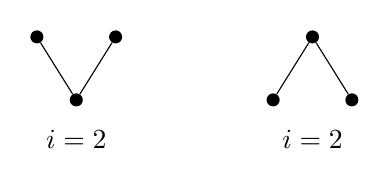
\begin{tikzpicture}
  \node[circle,fill=black,scale=0.5] (A1) at (1, 0) {};
  \node[circle,fill=black,scale=0.5] (A2) at (0.5, 0.8) {};
  \node[circle,fill=black,scale=0.5] (A3) at (1.5, 0.8) {};

  \draw (A1) -- (A2) node {};
  \draw (A1) -- (A3) node {};
  \node (AL) at (1, -0.5) {$i = 2$};


  \node[circle,fill=black,scale=0.5] (B1) at (3 + 1, 0.8) {};
  \node[circle,fill=black,scale=0.5] (B2) at (3 + 0.5, 0) {};
  \node[circle,fill=black,scale=0.5] (B3) at (3 + 1.5, 0) {};

  \draw (B1) -- (B2) node {};
  \draw (B1) -- (B3) node {};
  \node (BL) at (3 + 1, -0.5) {$i = 2$};
\end{tikzpicture}
%  \caption{According to \Cref{lemma:dual_poset_allowed}, the two posets are dual to each other.
%    However, \texttt{nauty} cannot be used to transform the posets into each other since they are different graphs.
%    This can also be seen in the Hasse diagram, which represents a directed graph, although the arrows are not shown here and always run implicitly from top to bottom.}
%  \label{fig:backward_canonify_problematic}
%\end{figure}
The next step is the computation of a hash value for each vertex in the poset.
We begin with the in- and out-degree for each vertex and assign a hash value based on these degrees.
Then, we iteratively update the hash value of each vertex, considering the hash value of the adjacent vertices.
Only three iterations are sufficient to obtain good-enough hash values.

The last step is to sort the vertices according to their hash values.
If all hash values are unique, we have a canonical labeling.
If there are vertices with the same hash, then we apply a special treatment to the following common situation.
Let there be $l$ non-overlapping pairs of vertices with identical hash values (and all other pairs have different hash values).
Then, there are $2^l$ possible permutations that could correspond to the normal form, since each of the $l$ pairs may or may not be swapped.
Given the realistic assumption that $l$ is small, all $2^l$ permutations can be efficiently iterated.
With the aim of obtaining values for $n = 16$, it follows that there are at most $\frac{n}{2}$ pairs, hence $l \leq 8$ always holds.
All $2^l$ posets are then calculated, and one permutation is deterministically selected based on its binary representation.
It should be noted that this special treatment only applies to pairs of two elements and no longer applies if there are three vertices with the same hash value.
All remaining ambiguous cases, not covered by the special treatment above, are handled using \texttt{nauty}.

In practice, our algorithm for computing the normal form rarely falls back to using \texttt{nauty}, as illustrated in \Cref{table:nauty-ratio}.
It is particularly noteworthy that as $i$ increases, the percentage of \texttt{nauty} calls decreases.
For small values of $i$, the high percentage of \texttt{nauty} calls is not critical, as computations for small $i$ are generally quick.

\begin{table}[!t]
  \renewcommand{\arraystretch}{1.1}
  \caption{Percentage of normal form computations using \texttt{nauty} for variable $n$ and $i$, where lower values are preferable.}
  \label{table:nauty-ratio}
  \centering
  \small
%  \resizebox{\columnwidth}{!}{%
    \begin{tabular}{cr|cccccccc}
%      $n$ & $i$ & \multicolumn{8}{c}{$i$}                                                          \\
      $n$ & $i$    & 1                       & 2      & 3     & 4     & 5     & 6     & 7     & 8     \\ \hline
      13 & & 0                       & 30.205 & 6.808 & 1.526 & 0.467 & 0.185 & 0.114 &       \\
      14 & & 0                       & 33.667 & 7.552 & 1.651 & 0.425 & 0.151 & 0.073 &       \\
      15 & & 0                       & 36.390 & 8.184 & 1.678 & 0.459 & 0.132 & 0.065 & 0.041 \\
      16 & & 0                       & 39.407 & 8.805 & 1.796 & 0.467 & 0.144 & -     & -     \\
    \end{tabular}%
%  }
\end{table}

\subsubsection{Optimizations.}

\subparagraph{Limit search space.}
Since there are potentially many predecessors that cannot contribute to the solution, they are not even calculated.
Many posets can be excluded based on $n$ and $i$.
For example, when searching for $n=7$ and $i=4$, only predecessors with certain properties are considered.
Specifically, only those predecessors that can lead to $n=7$, $i=4$ by adding a single comparison are relevant.

Adding a comparison can reduce n by a maximum of 1 and i by a maximum of 1.
Therefore, all other predecessors can be ignored, as they cannot contribute to the solution. 
For instance, no poset with $n=6$ and $i=2$ can lead to a poset with $n=7$, $i=4$.

\subparagraph{Remaining comparisons.}
In the next step, the minimum number of comparisons that must be removed until the unordered poset is reached is calculated for each predecessor.
This number corresponds to the edges in the corresponding Hasse diagram.
Since no more than one comparison can be removed in each step, all posets containing too many comparisons can be discarded, as they cannot lead to an unordered poset with the remaining comparisons.

\subparagraph{Iterative deepening.}
As the theoretical upper bounds are too high in practice, the program uses an iterative deepening approach.
It starts with an upper bound that corresponds to the theoretical lower bound, derived by \Cref{lemma:previous_next_poset} from the smaller values for $n$ and increments this bound until a solution is finally found.
As it is not possible to save which posets are lost due to the guessed upper bound without considerable effort, the backward search is restarted several times.
Although results from previous rounds are not used, the search space can be considerably reduced, making the program more efficient.

\subparagraph{Parallelization.} \label{sec:backward:parallelisation}
The backward search can be ideally parallelized by performing the calculation of the predecessors in parallel.
The only two bottlenecks here are read access to the cache and the efficient merging of all partial results.

\begin{table}[!t]
  \renewcommand{\arraystretch}{1.1}
  \caption{Efficiency of parallelism for $n = 13, i = 7$}
  \label{table:backward-parallel}
  \centering
  \small
  \begin{tabular}{l|rrrrrr}
    \textbf{cores}      & $1$    & $2$    & $3$    & $6$    & $12$   & $24$   \\ \hline
    \textbf{time} (m)   & 165    & 84     & 64     & 32     & 17     & 9      \\ \hline
    \textbf{efficiency} & $1.00$ & $0.99$ & $0.90$ & $0.87$ & $0.81$ & $0.75$
  \end{tabular}
\end{table}

As shown in \Cref{table:backward-parallel} for $n = 13$ and $i = 7$, it can be seen that the backward search scales well with the number of cores.
To set the different times in relation to the number of cores, the efficiency was determined, which represents a direct correlation between the two variables.
This can be calculated as follows
\[
  \text{efficiency} = \cfrac{\text{single-core time}}{\text{number of cores} \cdot \text{multi-core time}}
\]
The higher the efficiency, the better the time scales with the number of cores.

\begin{figure}[!b]
  \centering
  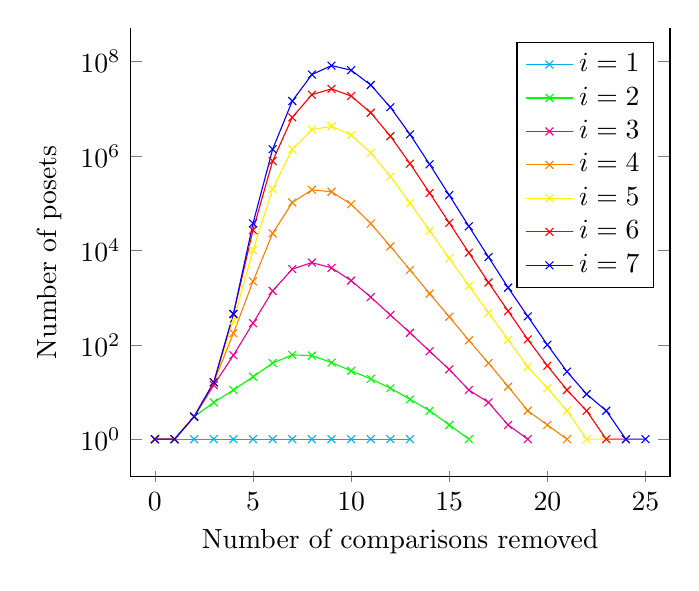
\begin{tikzpicture}
  \begin{axis}[
      ymode=log,
      axis x line = bottom,%x-Achse nur unten
      % x dir=reverse,
      enlarge x limits = .05,%x-Achse erweitern
      x axis line style = {-},%kein Pfeil
      % title = {\dots},
      ylabel={Number of posets},
      xlabel={Number of comparisons removed},
      % only marks,
      cycle list={{mark=x}},
      legend pos=north east,
    ]
    \addlegendentry{$i = 1$}
    \addplot+[cyan] table { %n=14,i=0
        x  y
        0  1
        1  1
        2  1
        3  1
        4  1
        5  1
        6  1
        7  1
        8  1
        9  1
        10 1
        11 1
        12 1
        13 1
      };
    \addlegendentry{$i = 2$}
    \addplot+[green] table { %n=14,i=1
        x y
        0  1
        1  1
        2  3
        3  6
        4  11
        5  21
        6  41
        7  61
        8  59
        9  42
        10 28
        11 19
        12 12
        13 7
        14 4
        15 2
        16 1
      };
    \addlegendentry{$i = 3$}
    \addplot+[magenta] table { %n=14,i=2
        x y
        0  1
        1  1
        2  3
        3  14
        4  60
        5  287
        6  1385
        7  4005
        8  5510
        9  4268
        10 2284
        11 1025
        12 428
        13 180
        14 73
        15 30
        16 11
        17 6
        18 2
        19 1
      };
    \addlegendentry{$i = 4$}
    \addplot+[orange] table { %n=14,i=3
        x y
        0  1
        1  1
        2  3
        3  16
        4  175
        5  2201
        6  22900
        7  103210
        8  191627
        9  174416
        10 94785
        11 37004
        12 12173
        13 3851
        14 1211
        15 392
        16 124
        17 41
        18 13
        19 4
        20 2
        21 1
      };
    \addlegendentry{$i = 5$}
    \addplot+[yellow] table { %n=14,i=4
        x y
        0  1
        1  1
        2  3
        3  16
        4  323
        5  10111
        6  200521
        7  1386176
        8  3607272
        9  4267576
        10 2763862
        11 1162696
        12 367875
        13 100552
        14 26024
        15 6745
        16 1781
        17 474
        18 127
        19 34
        20 12
        21 4
        22 1
        23 1
      };
    \addlegendentry{$i = 6$}
    \addplot+[red] table { %n=14,i=5
        x y
        0  1
        1  1
        2  3
        3  16
        4  446
        5  26921
        6  780123
        7  6588569
        8  19882832
        9  26416869
        10 18631911
        11 8243306
        12 2630332
        13 688904
        14 164372
        15 38334
        16 8918
        17 2084
        18 518
        19 130
        20 36
        21 11
        22 4
        23 1
        24 1
      };
    \addlegendentry{$i = 7$}
    \addplot+[blue] table { % n=14,i=6
        x y
        0  1
        1  1
        2  3
        3  16
        4  452
        5  37236
        6  1389385
        7  14591680
        8  53003482
        9  82198656
        10 65707713
        11 31909980
        12 10770689
        13 2864659
        14 665109
        15 147573
        16 32349
        17 7214
        18 1624
        19 400
        20 100
        21 27
        22 9
        23 4
        24 1
        25 1
      };
  \end{axis}
\end{tikzpicture}
  \caption{Number of posets generated by the backward search for $n = 14$ depending on the number of comparisons for various $i$.
    Be aware of the logarithmic scale of the y-axis and that the reverse search does not add comparisons, but rather removes them.}
  \label{fig:backward-posets-per-level}
\end{figure}

% todo: this paragraph is out of place!
\Cref{fig:backward-posets-per-level} shows the size of the search space of the backward search for different values of $i$.
It is noticeable that the maximum number of problems is searched for all $i$ when there are $8$ to $9$ comparisons remaining, with a slight tendency towards more comparisons for larger $i$ for $n = 14$.

\section{Results}

\begin{table}[!t]
  \renewcommand{\arraystretch}{1.1}
  \caption{Minimum number of comparisons needed to select the $i$-th smallest of $n$ elements.
    Values resulting from our work are printed in bold.}
  \label{table:num-comparisons}
  \centering
  \small
  \begin{tabular}{c|cccccccc}
    $n$ & \multicolumn{8}{c}{$i$}                                                                                                    \\
        & 1                       & 2  & 3           & 4           & 5           & 6           & 7                & 8                \\ \hline
    1   & 0                                                                                                                          \\
    2   & 1                                                                                                                          \\
    3   & 2                       & 3                                                                                                \\
    4   & 3                       & 4                                                                                                \\
    5   & 4                       & 6  & 6                                                                                           \\
    6   & 5                       & 7  & 8                                                                                           \\
    7   & 6                       & 8  & 10          & 10                                                                            \\
    8   & 7                       & 9  & 11          & 12                                                                            \\
    9   & 8                       & 11 & 12          & 14          & 14                                                              \\
    10  & 9                       & 12 & 14          & 15          & 16                                                              \\
    11  & 10                      & 13 & 15          & 17          & 18          & 18                                                \\
    12  & 11                      & 14 & 17          & 18          & 19          & 20                                                \\
    13  & 12                      & 15 & 18          & 20          & 21          & 22          & 23                                  \\
    14  & 13                      & 16 & 19          & 21          & 23          & 24          & \textbf{25}                         \\
    15  & 14                      & 17 & 20          & 23          & \textbf{24} & \textbf{26} & \textbf{26}      & \textbf{27}      \\
    16  & 15                      & 18 & \textbf{21} & \textbf{24} & \textbf{26} & \textbf{27} & \textbf{28} - 33 & \textbf{28} - 36 \\
  \end{tabular}
  \vspace{-\baselineskip}
\end{table}

Running our computer search, we obtained the values $V_i(n)$ shown in \Cref{table:num-comparisons}.
Our findings confirm most of the values computed by Oksanen~\cite{Oksanen}.
Notably, $V_5(12) = 19$ contradicts a conjecture by Gasarch~\cite{Gasarch1996} that the optimum can be achieved using a ``pair-forming algorithm'', where the first comparison of any singleton is with another singleton (in this case, the best pair-forming algorithm requires 20 comparisons).
The values printed in bold were unknown previously.
For $V_7(14)$, $V_6(15)$, $V_7(15)$, and $V_8(15)$, only a range was known prior.
Oksanen incorrectly lists $V_5(15)$ as 25 on his website~\cite{Oksanen}, although his search algorithm does produce the correct value of 24.
The values for $n = 16$ have not been computed before; we provide all values for $i \leq 6$ and ranges for $V_7(16)$ and $V_8(16)$.
The upper bound for the ranges is $V_i(n) \le n - i + (i - 1) \lceil \log (n + 2 - i) \rceil$~\cite{hadian1969selecting}.

\enlargethispage{\baselineskip}
To validate the upper bounds of the values we calculated, we checked the algorithm certifying each number on each of the $n!$ permutations.
Certifying the correctness of the lower bound is nearly impossible.
We computed each number twice using two different algorithms, the forward and the backward search.
Thus, it is unlikely that the results are incorrect due to a coding error.

\begin{table}[!t]
  \caption{Execution times for different search methods.}
  \label{table:search_algorithms}
\begin{minipage}{\linewidth}
  \renewcommand{\arraystretch}{1.1}
  \centering
  \small
  \begin{tabular}{c|c|l|l|l}
    $n$ & $i$ & \textbf{Forward} & \textbf{Backward} & \textbf{Oksanen} \\
    \hline
    12  & 6   & 1m 30s           & 18.0s             & 1.9s
            \\
    \hline
    13  & 7   & 59m 20s          & 7m 16s            & 16h 10m          \\
    \hline
    14  & 7   & 14h 40m          & 2h 17m            & >5d\footnote{\label{fn:oksanen_abort}We aborted Oksanen's program after 5 days.}   \\
    \hline
    15  & 8   & 14d 21h 26m      & 1d 3h 7m          & >5d\footref{fn:oksanen_abort}              \\
    \hline
    16  & 6   & 6d 11h 21m       & 1d 1h 26m         & -                \\
  \end{tabular}
  \end{minipage}
\end{table}

\Cref{table:search_algorithms} compares the execution times of the different algorithms to find optimal selection algorithms.
All experiments were conducted on a machine with two Intel Xeon CPUs, each equipped with $12$ cores ($24$ threads), and a total of $768$ GB of RAM.
The forward search was started with $500$ GB of RAM and restarted for each combination of $n$ and $i$, ensuring no use of cached data from previous runs to provide comparability.
The `Oksanen' column presents execution times of Oksanen's program~\cite{Oksanen} on our hardware, started with a cache size of $25$ GB RAM.
It was originally designed to use $400$ MB RAM and $25$ GB is close to a natural limit due to the use of 32-bit indices.
Additionally, we measured the number of posets stored in the cache after the calculation, which can be found in \Cref{table:cache_entries}.


\begin{table}[!t]
  \renewcommand{\arraystretch}{1.1}
  \caption{Number of posets stored in the cache after the corresponding search}
  \label{table:cache_entries}
  \centering
  \small
  \begin{tabular}{c|c|r|r}
    $n$ & $i$ & \textbf{Forward Search} & \textbf{Backward Search} \\
    \hline
    13  & 7   & $67.6 \cdot 10^6$       & $14.5 \cdot 10^6$        \\
    \hline
    14  & 7   & $925.3 \cdot 10^6$      & $263.3 \cdot 10^6$       \\
    \hline
    15  & 8   & $15.7 \cdot 10^9$       & $2.2 \cdot 10^9$         \\
    \hline
    16  & 6   & $3.6 \cdot 10^9$        & $2.6 \cdot 10^9$         \\
  \end{tabular}
\end{table}

To evaluate the potential of compatible solutions as pruning criterion, we determined the maximum number of compatible solutions encountered for a given cost for $n \leq 14$ and used that as a boundary in a subsequent run.
For $n = 14, i = 7$, this resulted in a time of 1h~21m with $147 \cdot 10^6$ posets in the cache, representing improvements by factors of $11$ and $6.3$, respectively.


\section{Conclusion and Open Questions}


As stated in the motivation before: the road is better than the inn.
Along the way we improved the forward search using a pruning criterion based on compatible solutions and evaluated a new algorithmic approach -- the backward search coming to a final conclusion that both are valid.
Between the structural constraints of our algorithms and the available hardware, $n=16$ is likely the limit of feasible calculation for the current state.
We believe that higher $n$ are realistic with new algorithmic ideas and conclude this work by talking about promising directions for further research.
The latest version of our software is available at \projectServer~(\url{\projectURL}).

\subparagraph{Bidirectional Search.}
The classical meet-in-the-middle approach for a bidirectional search will not work for the selection problem.
This is illustrated in \Cref{fig:backward_forward_count_13_6}:
Assume the two searches meet after $11$ comparisons have been performed.
At this meeting point, both searches have already covered over $99\%$ of their search space.

\begin{figure}[!b]
  \centering
  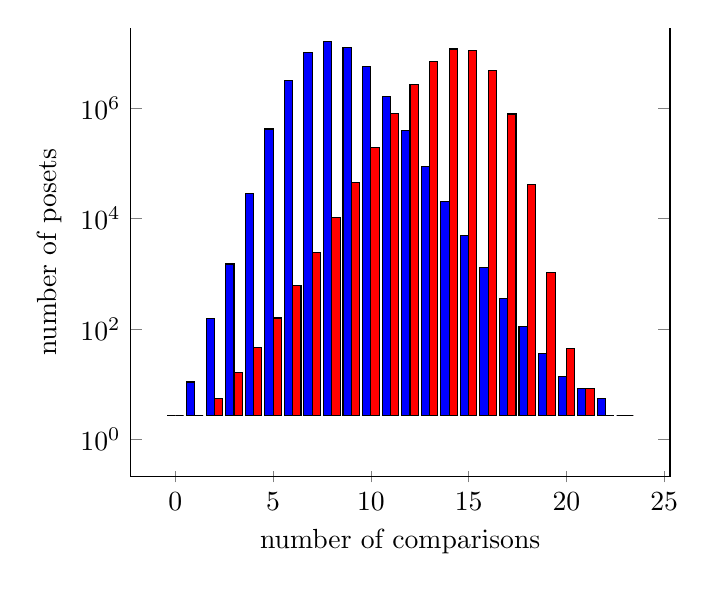
\begin{tikzpicture}
  \begin{axis}[
      ybar,
      ymode=log,
      axis x line = bottom,%x-Achse nur unten
      enlarge x limits = .1,%x-Achse erweitern
      x axis line style = {-},%kein Pfeil
      bar width=3pt,
      ylabel={number of posets},
      xlabel={number of comparisons},
      % legend cell align=left,
      % legend pos=outer north east,
      % legend style={at={(0.5,-0.2)},anchor=north}, % draw=none
    ]
    % \addlegendentry{forward search}
    \addplot[fill=blue,shift={(1pt, 0)}] table {
        x y
        0  1
        1  4
        2  57
        3  552
        4  10397
        5  154828
        6  1166640
        7  3770182
        8  5941732
        9  4726819
        10 2096404
        11 604582
        12 143058
        13 32460
        14 7450
        15 1823
        16 471
        17 132
        18 41
        19 13
        20 5
        21 3
        22 2
        23 1
      };
    % \addlegendentry{backward search}
    \addplot[fill=red,shift={(-1pt, 0)}] table {
        x y
        23 1
        22 1
        21 3
        20 16
        19 381
        18 15227
        17 290138
        16 1750707
        15 4058631
        14 4368185
        13 2592437
        12 1006071
        11 291970
        10 72346
        9  16728
        8  3898
        7  893
        6  227
        5  58
        4  17
        3  6
        2  2
        1  1
        0  1
      };
  \end{axis}
\end{tikzpicture}

Treff: 11
  \caption{Number of posets depending on the number of comparisons for $n = 13$ and $i = 7$ (red: backward search, blue: forward search).}
  \label{fig:backward_forward_count_13_6}
\end{figure}

An alternative approach to the bidirectional search would be to first run the backward search, but restrict it to problems with specific properties such as having a large number of compatible solutions, e.g.\ problems $(P, i)$ in $A_k$ with $\mathcal{C}(P, i) \ge \alpha \cdot 2^k$ for some $\alpha \in [0, 1]$.
These are presumably hard to solve, so the subsequent forward search only has to explore problems with a small number of compatible solutions, which we estimate to be easier to solve.

There might be better metrics than the compatible solutions, as there is a significant gap between the lower bound and the cost of a problem.
We observed that the number of comparisons required to solve a selection problem is typically about twice the lower bound obtained from the number of compatible solutions, minus a constant.
This observation is reasonable, as the lower bound for the median is $n + \smallO(n)$, which is far from the best known asymptotic lower bound $2n + \smallO(n)$.

\subparagraph{Improved Weight Function.}
A better lower bound might be achieved by assigning a weight to each solution rather than merely counting compatible solutions.
%It is relatively straightforward to create a weight function that leads to a lower bound of $1.5n + \smallO(n)$ for the median.
Mimicking the techniques used to obtain the $2n + \smallO(n)$ bound in~\cite{bent1985finding} could be a fruitful approach.
%However, this lead to a negative $4\sqrt{n}$ term in the resulting lower bound for $n \leq 16$, cancelling out any improvement over counting compatible solutions.
%\enlargethispage{\baselineskip}

\subparagraph{Yao's conjecture.}
Yao conjectured that finding the $i$-th smallest of $n$ elements is at least as hard as finding an $n$-element subset $S$ of $m$ elements, where $m > n$, and an element $s \in S$ such that $s$ is the $i$-th smallest element in $S$~\cite{yao1974lower}.
If true, it would imply a $2.5n + \smallO(n)$ algorithm for computing the median~\cite{schonhage1975finding}.
By adapting our search algorithm, one could search for counter examples to the conjecture.

\clearpage

% =====================================================

% \section{Typesetting instructions -- Summary}
% \label{sec:typesetting-summary}

% LIPIcs is a series of open access high-quality conference proceedings across all fields in informatics established in cooperation with Schloss Dagstuhl. 
% In order to do justice to the high scientific quality of the conferences that publish their proceedings in the LIPIcs series, which is ensured by the thorough review process of the respective events, we believe that LIPIcs proceedings must have an attractive and consistent layout matching the standard of the series.
% Moreover, the quality of the metadata, the typesetting and the layout must also meet the requirements of other external parties such as indexing service, DOI registry, funding agencies, among others. The guidelines contained in this document serve as the baseline for the authors, editors, and the publisher to create documents that meet as many different requirements as possible. 

% Please comply with the following instructions when preparing your article for a LIPIcs proceedings volume. 
% \paragraph*{Minimum requirements}

% \begin{itemize}
% \item Use pdflatex and an up-to-date \LaTeX{} system.
% \item Use further \LaTeX{} packages and custom made macros carefully and only if required.
% \item Use the provided sectioning macros: \verb+\section+, \verb+\subsection+, \verb+\subsubsection+, \linebreak \verb+\paragraph+, \verb+\paragraph*+, and \verb+\subparagraph*+.
% \item Provide suitable graphics of at least 300dpi (preferably in PDF format).
% \item Use BibTeX and keep the standard style (\verb+plainurl+) for the bibliography.
% \item Please try to keep the warnings log as small as possible. Avoid overfull \verb+\hboxes+ and any kind of warnings/errors with the referenced BibTeX entries.
% \item Use a spellchecker to correct typos.
% \end{itemize}

% \paragraph*{Mandatory metadata macros}
% Please set the values of the metadata macros carefully since the information parsed from these macros will be passed to publication servers, catalogues and search engines.
% Avoid placing macros inside the metadata macros. The following metadata macros/environments are mandatory:
% \begin{itemize}
% \item \verb+\title+ and, in case of long titles, \verb+\titlerunning+.
% \item \verb+\author+, one for each author, even if two or more authors have the same affiliation.
% \item \verb+\authorrunning+ and \verb+\Copyright+ (concatenated author names)\\
% The \verb+\author+ macros and the \verb+\Copyright+ macro should contain full author names (especially with regard to the first name), while \verb+\authorrunning+ should contain abbreviated first names.
% \item \verb+\ccsdesc+ (ACM classification, see \url{https://www.acm.org/publications/class-2012}).
% \item \verb+\keywords+ (a comma-separated list of keywords).
% \item \verb+\relatedversion+ (if there is a related version, typically the ``full version''); please make sure to provide a persistent URL, e.\,g., at arXiv.
% \item \verb+\begin{abstract}...\end{abstract}+ .
% \end{itemize}

% \paragraph*{Please do not \ldots} %Do not override the \texttt{\seriesstyle}-defaults}
% Generally speaking, please do not override the \texttt{lipics-v2021}-style defaults. To be more specific, a short checklist also used by Dagstuhl Publishing during the final typesetting is given below.
% In case of \textbf{non-compliance} with these rules Dagstuhl Publishing will remove the corresponding parts of \LaTeX{} code and \textbf{replace it with the \texttt{lipics-v2021} defaults}. In serious cases, we may reject the LaTeX-source and expect the corresponding author to revise the relevant parts.
% \begin{itemize}
% \item Do not use a different main font. (For example, the \texttt{times} package is forbidden.)
% \item Do not alter the spacing of the \texttt{lipics-v2021.cls} style file.
% \item Do not use \verb+enumitem+ and \verb+paralist+. (The \texttt{enumerate} package is preloaded, so you can use
%  \verb+\begin{enumerate}[(a)]+ or the like.)
% \item Do not use ``self-made'' sectioning commands (e.\,g., \verb+\noindent{\bf My+ \verb+Paragraph}+).
% \item Do not hide large text blocks using comments or \verb+\iffalse+ $\ldots$ \verb+\fi+ constructions. 
% \item Do not use conditional structures to include/exclude content. Instead, please provide only the content that should be published -- in one file -- and nothing else.
% \item Do not wrap figures and tables with text. In particular, the package \texttt{wrapfig} is not supported.
% \item Do not change the bibliography style. In particular, do not use author-year citations. (The
% \texttt{natbib} package is not supported.)
% \end{itemize}

% \enlargethispage{\baselineskip}

% This is only a summary containing the most relevant details. Please read the complete document ``LIPIcs: Instructions for Authors and the \texttt{lipics-v2021} Class'' for all details and don't hesitate to contact Dagstuhl Publishing (\url{mailto:publishing@dagstuhl.de}) in case of questions or comments:
% \href{http://drops.dagstuhl.de/styles/lipics-v2021/lipics-v2021-authors/lipics-v2021-authors-guidelines.pdf}{\texttt{http://drops.dagstuhl.de/styles/lipics-v2021/\newline lipics-v2021-authors/lipics-v2021-authors-guidelines.pdf}}

% \section{Lorem ipsum dolor sit amet}

% Lorem ipsum dolor sit amet, consectetur adipiscing elit \cite{DBLP:journals/cacm/Knuth74}. Praesent convallis orci arcu, eu mollis dolor. Aliquam eleifend suscipit lacinia. Maecenas quam mi, porta ut lacinia sed, convallis ac dui. Lorem ipsum dolor sit amet, consectetur adipiscing elit. Suspendisse potenti. Donec eget odio et magna ullamcorper vehicula ut vitae libero. Maecenas lectus nulla, auctor nec varius ac, ultricies et turpis. Pellentesque id ante erat. In hac habitasse platea dictumst. Curabitur a scelerisque odio. Pellentesque elit risus, posuere quis elementum at, pellentesque ut diam. Quisque aliquam libero id mi imperdiet quis convallis turpis eleifend. 

% \begin{lemma}[Lorem ipsum]
% \label{lemma:lorem}
% Vestibulum sodales dolor et dui cursus iaculis. Nullam ullamcorper purus vel turpis lobortis eu tempus lorem semper. Proin facilisis gravida rutrum. Etiam sed sollicitudin lorem. Proin pellentesque risus at elit hendrerit pharetra. Integer at turpis varius libero rhoncus fermentum vitae vitae metus.
% \end{lemma}

% \begin{proof}
% Cras purus lorem, pulvinar et fermentum sagittis, suscipit quis magna.


% \proofsubparagraph*{Just some paragraph within the proof.}
% Nam liber tempor cum soluta nobis eleifend option congue nihil imperdiet doming id quod mazim placerat facer possim assum. Lorem ipsum dolor sit amet, consectetuer adipiscing elit, sed diam nonummy nibh euismod tincidunt ut laoreet dolore magna aliquam erat volutpat.
% \begin{claim}
% content...
% \end{claim}
% \begin{claimproof}
% content...
%     \begin{enumerate}
%         \item abc abc abc \claimqedhere{}
%     \end{enumerate}
% \end{claimproof}

% \end{proof}

% \begin{corollary}[Curabitur pulvinar, \cite{DBLP:books/mk/GrayR93}]
% \label{lemma:curabitur}
% Nam liber tempor cum soluta nobis eleifend option congue nihil imperdiet doming id quod mazim placerat facer possim assum. Lorem ipsum dolor sit amet, consectetuer adipiscing elit, sed diam nonummy nibh euismod tincidunt ut laoreet dolore magna aliquam erat volutpat.
% \end{corollary}

% \begin{proposition}\label{prop1}
% This is a proposition
% \end{proposition}

% \autoref{prop1} and \cref{prop1} \ldots

% \subsection{Curabitur dictum felis id sapien}

% Curabitur dictum \cref{lemma:curabitur} felis id sapien \autoref{lemma:curabitur} mollis ut venenatis tortor feugiat. Curabitur sed velit diam. Integer aliquam, nunc ac egestas lacinia, nibh est vehicula nibh, ac auctor velit tellus non arcu. Vestibulum lacinia ipsum vitae nisi ultrices eget gravida turpis laoreet. Duis rutrum dapibus ornare. Nulla vehicula vulputate iaculis. Proin a consequat neque. Donec ut rutrum urna. Morbi scelerisque turpis sed elit sagittis eu scelerisque quam condimentum. Pellentesque habitant morbi tristique senectus et netus et malesuada fames ac turpis egestas. Aenean nec faucibus leo. Cras ut nisl odio, non tincidunt lorem. Integer purus ligula, venenatis et convallis lacinia, scelerisque at erat. Fusce risus libero, convallis at fermentum in, dignissim sed sem. Ut dapibus orci vitae nisl viverra nec adipiscing tortor condimentum \cite{DBLP:journals/cacm/Dijkstra68a}. Donec non suscipit lorem. Nam sit amet enim vitae nisl accumsan pretium. 

% \begin{lstlisting}[caption={Useless code.},label=list:8-6,captionpos=t,float,abovecaptionskip=-\medskipamount]
% for i:=maxint to 0 do 
% begin 
%     j:=square(root(i));
% end;
% \end{lstlisting}

% \subsection{Proin ac fermentum augue}

% Proin ac fermentum augue. Nullam bibendum enim sollicitudin tellus egestas lacinia euismod orci mollis. Nulla facilisi. Vivamus volutpat venenatis sapien, vitae feugiat arcu fringilla ac. Mauris sapien tortor, sagittis eget auctor at, vulputate pharetra magna. Sed congue, dui nec vulputate convallis, sem nunc adipiscing dui, vel venenatis mauris sem in dui. Praesent a pretium quam. Mauris non mauris sit amet eros rutrum aliquam id ut sapien. Nulla aliquet fringilla sagittis. Pellentesque eu metus posuere nunc tincidunt dignissim in tempor dolor. Nulla cursus aliquet enim. Cras sapien risus, accumsan eu cursus ut, commodo vel velit. Praesent aliquet consectetur ligula, vitae iaculis ligula interdum vel. Integer faucibus faucibus felis. 

% \begin{itemize}
% \item Ut vitae diam augue. 
% \item Integer lacus ante, pellentesque sed sollicitudin et, pulvinar adipiscing sem. 
% \item Maecenas facilisis, leo quis tincidunt egestas, magna ipsum condimentum orci, vitae facilisis nibh turpis et elit. 
% \end{itemize}

% \begin{remark}
% content...
% \end{remark}

% \section{Pellentesque quis tortor}

% Nec urna malesuada sollicitudin. Nulla facilisi. Vivamus aliquam tempus ligula eget ornare. Praesent eget magna ut turpis mattis cursus. Aliquam vel condimentum orci. Nunc congue, libero in gravida convallis \cite{DBLP:conf/focs/HopcroftPV75}, orci nibh sodales quam, id egestas felis mi nec nisi. Suspendisse tincidunt, est ac vestibulum posuere, justo odio bibendum urna, rutrum bibendum dolor sem nec tellus. 

% \begin{lemma} [Quisque blandit tempus nunc]
% Sed interdum nisl pretium non. Mauris sodales consequat risus vel consectetur. Aliquam erat volutpat. Nunc sed sapien ligula. Proin faucibus sapien luctus nisl feugiat convallis faucibus elit cursus. Nunc vestibulum nunc ac massa pretium pharetra. Nulla facilisis turpis id augue venenatis blandit. Cum sociis natoque penatibus et magnis dis parturient montes, nascetur ridiculus mus.
% \end{lemma}

% Fusce eu leo nisi. Cras eget orci neque, eleifend dapibus felis. Duis et leo dui. Nam vulputate, velit et laoreet porttitor, quam arcu facilisis dui, sed malesuada risus massa sit amet neque.

% \section{Morbi eros magna}

% Morbi eros magna, vestibulum non posuere non, porta eu quam. Maecenas vitae orci risus, eget imperdiet mauris. Donec massa mauris, pellentesque vel lobortis eu, molestie ac turpis. Sed condimentum convallis dolor, a dignissim est ultrices eu. Donec consectetur volutpat eros, et ornare dui ultricies id. Vivamus eu augue eget dolor euismod ultrices et sit amet nisi. Vivamus malesuada leo ac leo ullamcorper tempor. Donec justo mi, tempor vitae aliquet non, faucibus eu lacus. Donec dictum gravida neque, non porta turpis imperdiet eget. Curabitur quis euismod ligula. 


%%
%% Bibliography
%%

%% Please use bibtex, 

\bibliography{lipics-v2021-sample-article}

\clearpage
\appendix

\section{Example.}
% todo: Can we make this smaller / same style as the other figures?
\begin{figure}[!b]
  \centering
  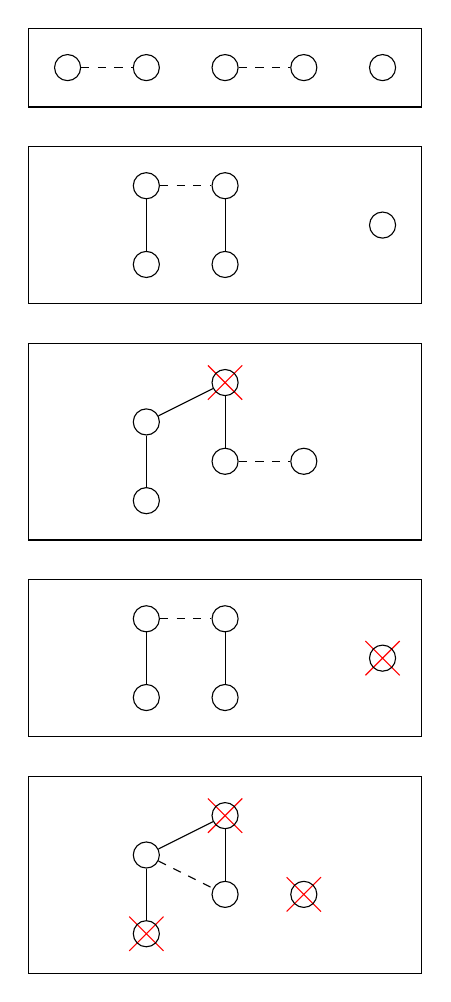
\begin{tikzpicture}[tcancel/.append style={draw=#1, cross out, inner sep=6pt}]
  \draw(-.5, -.5) rectangle (4.5, .5);
  \node[circle,draw=black] (A1) at (0, 0) {};
  \node[circle,draw=black] (A2) at (1, 0) {};
  \node[circle,draw=black] (A3) at (2, 0) {};
  \node[circle,draw=black] (A4) at (3, 0) {};
  \node[circle,draw=black] (A5) at (4, 0) {};

  \draw[dashed] (A1) -- (A2) node {};
  \draw[dashed] (A3) -- (A4) node {};

  \draw(-0.5, -3.0) rectangle (4.5, -1.0);
  \node[circle,draw=black] (B1) at (1.0, 0 - 2.5) {};
  \node[circle,draw=black] (B2) at (1.0, 1 - 2.5) {};
  \node[circle,draw=black] (B3) at (2.0, 0 - 2.5) {};
  \node[circle,draw=black] (B4) at (2.0, 1 - 2.5) {};
  \node[circle,draw=black] (B5) at (4.0, 0.5 - 2.5) {};

  \draw (B1) -- (B2) node {};
  \draw (B3) -- (B4) node {};
  \draw[dashed] (B2) -- (B4) node {};

  \draw(-0.5, -6.0) rectangle (4.5, -3.5);
  \node[circle,draw=black] (C1) at (1, 0 - 5.5) {};
  \node[circle,draw=black] (C2) at (1, 1 - 5.5) {};
  \node[circle,draw=black,tcancel=red] (C3) at (2, 1.5 - 5.5) {};
  \node[circle,draw=black] (C3) at (2, 1.5 - 5.5) {};
  \node[circle,draw=black] (C4) at (2, .5 - 5.5) {};
  \node[circle,draw=black] (C5) at (3, .5 - 5.5) {};

  \draw (C1) -- (C2) node {};
  \draw (C3) -- (C4) node {};
  \draw (C2) -- (C3) node {};
  \draw[dashed] (C4) -- (C5) node {};

  \draw(-0.5, -8.5) rectangle (4.5, -6.5);
  \node[circle,draw=black] (D1) at (1.0, 0 - 8) {};
  \node[circle,draw=black] (D2) at (1.0, 1 - 8) {};
  \node[circle,draw=black] (D3) at (2.0, 0 - 8) {};
  \node[circle,draw=black] (D4) at (2.0, 1 - 8) {};
  \node[circle,draw=black,tcancel=red] (D5) at (4.0, 0.5 - 8) {};
  \node[circle,draw=black] (D5) at (4.0, 0.5 - 8) {};

  \draw (D1) -- (D2) node {};
  \draw (D3) -- (D4) node {};
  \draw[dashed] (D2) -- (D4) node {};

  \draw(-0.5, -11.5) rectangle (4.5, -9.);
  \node[circle,draw=black,tcancel=red] (E1) at (1, 0 - 11.0) {};
  \node[circle,draw=black] (E1) at (1, 0 - 11.0) {};
  \node[circle,draw=black] (E2) at (1, 1 - 11.0) {};
  \node[circle,draw=black,tcancel=red] (E3) at (2, 1.5 - 11.0) {};
  \node[circle,draw=black] (E3) at (2, 1.5 - 11.0) {};
  \node[circle,draw=black] (E4) at (2, .5 - 11.0) {};
  \node[circle,draw=black,tcancel=red] (E5) at (3, .5 - 11.0) {};
  \node[circle,draw=black] (E5) at (3, .5 - 11.0) {};

  \draw (E1) -- (E2) node {};
  \draw (E3) -- (E4) node {};
  \draw (E2) -- (E3) node {};
  \draw[dashed] (E2) -- (E4) node {};
\end{tikzpicture}
  \caption{Finding the median $i = 3$ of $n = 5$ values using six comparisons.}
  \label{fig:median_of_5}
\end{figure}

A good visual example is finding the median $i = 3$ in a list of $n = 5$ elements.
\Cref{fig:median_of_5} illustrates the search process of finding the median using Hasse diagrams.
Each step shows the comparisons to be performed next, indicated by dashed lines.
A Hasse diagram of the order relation found so far (with smaller elements positioned lower and larger elements higher) is shown with solid lines.
The red crosses indicate elements that have been found to be greater or smaller than three other elements, thereby disqualifying them from being the median.
The larger element of the final comparison is the median.
This is also the optimal algorithm for $i = 3$ and $n = 5$.


% todo: Details on how potential predecessors are computed (especially regarding transitive relations).

% todo: Approximate normal form for forward search.

\section{Execution time and number of posets stored.}

\begin{table}[!t]
  \caption{Execution times of different search methods.}
  \label{table:search_algorithms_appendix}

\begin{minipage}{\linewidth}
  \renewcommand{\arraystretch}{1.1}
  \centering
  \small
  \begin{tabular}{c|c|l|l|l}
    $n$ & $i$ & \textbf{Forward} & \textbf{Backward} & \textbf{Oksanen} \\
    \hline
    12  & 1   & 0.0s             & 0.0s              & 0.0s             \\
    12  & 2   & 0.0s             & 0.2s              & 0.0s             \\
    12  & 3   & 0.4s             & 0.6s              & 0.0s             \\
    12  & 4   & 3.5s             & 0.9s              & 21.4s\footnote{\label{fn:oksanen_incorrect}The publicly available version \texttt{1.6} of Oksanen's program did not find an optimal algorithm for $V_4(12)$, $V_5(12)$ and $V_6(12)$. On his website he gives an optimal algorithm computed with the unavailable version \texttt{1.1}.}           \\
    12  & 5   & 36.1s            & 3.8s              & 4m 59s\footref{fn:oksanen_incorrect}
          \\
    12  & 6   & 1m 30s           & 18.0s             & 1.9s\footref{fn:oksanen_incorrect}
            \\
    \hline
    13  & 1   & 0.0s             & 0.0s              & 0.0s             \\
    13  & 2   & 0.0s             & 0.5s              & 0.0s             \\
    13  & 3   & 0.8s             & 1.2s              & 0.2s             \\
    13  & 4   & 13.8s            & 10.3s             & 55.4s            \\
    13  & 5   & 3m 42s           & 44.5s             & 26m 36s          \\
    13  & 6   & 17m 10s          & 3m 22s            & 3h 25m           \\
    13  & 7   & 59m 20s          & 7m 16s            & 16h 10m          \\
    \hline
    14  & 1   & 0.0s             & 0.0s              & 0.0s             \\
    14  & 2   & 0.0s             & 1.3s              & 0.0s             \\
    14  & 3   & 1.4s             & 5.1s              & 0.6s             \\
    14  & 4   & 35.9s            & 33.0s             & 1m 47s           \\
    14  & 5   & 17m 27s          & 7m 1s             & 6h 29m           \\
    14  & 6   & 2h 40m           & 37m 54s           & 4d 10h           \\
    14  & 7   & 14h 40m          & 2h 17m            & >5d\footnote{\label{fn:oksanen_abort_appendix}We aborted Oksanen's program after 5 days.}   \\
    \hline
    15  & 1   & 0.0s             & 0.0s              & 0.0s             \\
    15  & 2   & 0.1s             & 3.9s              & 0.0s             \\
    15  & 3   & 2.8s             & 24.5s             & 1.4s             \\
    15  & 4   & 2m 24s           & 11m 2s            & 27m 17s          \\
    15  & 5   & 1h 12m           & 22m 11s           & 1d 5h 40m        \\
    15  & 6   & 1d 8h 37m        & 7h 17m            & >5d\footref{fn:oksanen_abort}              \\
    15  & 7   & 4d 23h 37m       & 9h 45m            & >5d\footref{fn:oksanen_abort}              \\
    15  & 8   & 14d 21h 26m      & 1d 3h 7m          & >5d\footref{fn:oksanen_abort}              \\
    \hline
    16  & 1   & 0.0s             & 0.0s              & -                \\
    16  & 2   & 0.2s             & 12.3s             & -                \\
    16  & 3   & 6.4s             & 1m 55.1s          & -                \\
    16  & 4   & 7m 22s           & 52m 9.4s          & -                \\
    16  & 5   & 7h 33m           & 6h 48m 14.8s      & -                \\
    16  & 6   & 6d 11h 21m       & 1d 1h 26m         & -                \\ 
  \end{tabular}
  \end{minipage}
\end{table}


\begin{table}[!t]
  \renewcommand{\arraystretch}{1.1}
  \caption{Number of posets stored in the cache after the corresponding search}
  \label{table:cache_entries_appendix}
  \centering
  \small
  \begin{tabular}{c|c|r|r}
    $n$ & $i$ & \textbf{Forward Search} & \textbf{Backward Search} \\
    \hline
    13  & 1   & $12$                    & $13$                     \\
    13  & 2   & $329$                   & $245$                    \\
    13  & 3   & $9.7 \cdot 10^3$        & $10.9 \cdot 10^3$        \\
    13  & 4   & $199.7 \cdot 10^3$      & $276.9 \cdot 10^3$       \\
    13  & 5   & $3.7 \cdot 10^6$        & $2.2 \cdot 10^6$         \\
    13  & 6   & $18.1 \cdot 10^6$       & $9.7 \cdot 10^6$         \\
    13  & 7   & $67.6 \cdot 10^6$       & $14.5 \cdot 10^6$        \\
    \hline
    14  & 1   & $13$                    & $14$                     \\
    14  & 2   & $442$                   & $319$                    \\
    14  & 3   & $15.2 \cdot 10^3$       & $19.6 \cdot 10^3$        \\
    14  & 4   & $438.0 \cdot 10^3$      & $644.2 \cdot 10^3$       \\
    14  & 5   & $14.1 \cdot 10^6$       & $13.9 \cdot 10^6$        \\
    14  & 6   & $149.5 \cdot 10^6$      & $84.1 \cdot 10^6$        \\
    14  & 7   & $925.3 \cdot 10^6$      & $263.3 \cdot 10^6$       \\
    \hline
    15  & 1   & $14$                    & $15$                     \\
    15  & 2   & $741$                   & $407$                    \\
    15  & 3   & $23.6 \cdot 10^3$       & $34.9 \cdot 10^3$        \\
    15  & 4   & $1.3 \cdot 10^6$        & $3.1 \cdot 10^6$         \\
    15  & 5   & $53.0 \cdot 10^6$       & $40.0 \cdot 10^6$        \\
    15  & 6   & $1.6 \cdot 10^9$        & $0.73 \cdot 10^9$        \\
    15  & 7   & $5.3 \cdot 10^9$        & $1.3 \cdot 10^9$         \\
    15  & 8   & $15.7 \cdot 10^9$       & $2.2 \cdot 10^9$         \\
    \hline
    16  & 1   & $15$                    & $16$                     \\
    16  & 2   & $990$                   & $520$                    \\
    16  & 3   & $35.8 \cdot 10^3$       & $62.3 \cdot 10^3$        \\
    16  & 4   & $2.4 \cdot 10^6$        & $7.4 \cdot 10^6$         \\
    16  & 5   & $211.1 \cdot 10^6$      & $275.3 \cdot 10^6$       \\
    16  & 6   & $3.6 \cdot 10^9$        & $2.6 \cdot 10^9$         \\
  \end{tabular}
\end{table}




\section{Hard- and Software Used.} \label{sec:hardware}

Our results were facilitated by advancements in both hardware and software.
All versions of the software used are listed in \Cref{table:command_outputs}.
For hardware, we employed two Intel Xeon E5-2650v4 CPUs (2.20\,GHz, 12 Cores/24 Threads, 30\,MB L3-Cache per CPU), and a total of $768$ GB of RAM.

\begin{table}[!t]
  \renewcommand{\arraystretch}{1.1}
  \caption{Specific versions of the software used.}
  \label{table:command_outputs}
  \centering
  \small
  \begin{tabular}{l|l}
    \textbf{Command}  & \textbf{Output}                   \\ \hline
    \texttt{rustc -V} & rustc 1.77.2                      \\ \hline
    \texttt{clang -v} & Ubuntu clang version 14.0.0-1     \\ \hline
    \texttt{uname -a} & Linux plankton 5.15.0-105-generic \\
  \end{tabular}
\end{table}

\section{Distribution of Compatible Solutions}

\begin{figure}[h]
  \includegraphics*[scale=0.5]{figures/compatible_cost_relation.png}
  \caption*{Cost distribution for all instances solved in the forward search for $n \leq 14$, excluding $i \leq 2$.
    Purple indicates low $i$, yellow indicates high $i$. $\log_2$ is shown in red.}
\end{figure}

\section{ComputingCompatible Solutions.}
\Cref{algo:compatible_solutions} shows how we compute the number of compatible solutions for a given problem.
To calculate this number, the algorithm first picks a solution element $j$ -- since problems are always reduced in the forward search, any element is valid -- and then counts the number of partitions into greater and lesser elements, summing these counts over all solution elements.
The algorithm assumes that the elements in the poset are sorted such that an element smaller than another has a smaller index.

\begin{algorithm}[t]
  \centering
  \begin{algorithmic}

    \Function{NumCompatibleSolutions}{$(P, i)$}

    \State{$c \gets 0$}

    \For{$j \in \Omega_P$} \Comment{solutions with $j$ $i$-th smallest}

    \State{$\mathcal{D} \gets \{ \less{P}{j} \setminus \{j\} \}$}% \Comment{downsets containing $\less{P}{j} \setminus \{j\}$}

    \For{$k \in \Omega_P \setminus (\less{P}{j} \cup \greater{P}{j})$}

    \For{$S \in \mathcal{D}$}

    \If{$\less{P}{k} \subseteq S \cup \{ k \}$}
    \State{$\mathcal{D} \gets \mathcal{D} \cup \{ S \cup \{ k \} \}$}
    \EndIf

    \EndFor

    \EndFor

    \State{$c \gets c + |\{S \in \mathcal{D} \mid |S| = i \}|$}

    \EndFor

    \State{\Return{$c$}}

    \EndFunction
\end{algorithmic}

% New Version

% pub fn num_compatible_posets(&self) -> usize {
% debug_assert!(self.is_lower_triangle_matrix());

% let all_less_than = {
%     let mut bitsets = [BitSet::empty(); MAX_N];
%     bitsets
%         .iter_mut()
%         .take(self.n() as usize)
%         .enumerate()
%         .for_each(|(i, bs)| *bs = self.get_all_less_than(i as u8));
%     bitsets
% };

% let mut less_subsets = Vec::with_capacity(1000);

% let mut sum = 0;
% for i in 0..self.n() as usize {
%     // assume the ith element is the solution

%     let less_than_i = all_less_than[i];

%     if less_than_i.len() == self.i() as usize {
%         sum += 1;
%         continue;
%     }
%     if less_than_i.len() > self.i() as usize {
%         continue;
%     }

%     let greater_than_i = self.get_all_greater_than(i as u8);
%     let ordered_with_i = less_than_i.union(greater_than_i);

%     less_subsets.clear();
%     less_subsets.push(less_than_i);

%     for j in 0..self.n() as usize {
%         if j == i || ordered_with_i.contains(j) {
%             continue;
%         }

%         let less_than_j = all_less_than[j];

%         // try adding j to all previous subsets
%         for i in 0..less_subsets.len() {
%             let subset = less_subsets[i];

%             // test if adding j would make a valid subset
%             // we know, that there is no k with p[k] > p[j]
%             if less_than_j.intersect(subset) == less_than_j {
%                 let mut new_subset = subset;
%                 new_subset.insert(j);
%                 less_subsets.push(new_subset);
%             }
%         }
%     }

%     sum += less_subsets
%         .iter()
%         .filter(|s| s.len() == self.i() as usize)
%         .count();
% }

% sum
% }

% Old Version

% pub fn num_compatible_posets(&self) -> usize {
%     let canonified = self.canonify_lower_matrix();

%     let mut sum = 0;
%     for i in 0..canonified.n {
%         // assume the ith element is the solution

%         let less_than_i = canonified.get_all_less_than(i);
%         let greater_than_i = canonified.get_all_greater_than(i);

%         let mut less_subsets = Vec::new();
%         less_subsets.push(BitSet::empty());

%         for j in 0..canonified.n {
%             if j == i || greater_than_i.contains(j as usize) {
%                 continue;
%             }

%             let less_than_j = canonified.get_all_less_than(j);

%             // try adding j to all previous subsets
%             if less_than_i.contains(j as usize) {
%                 // all subsets must contain j to be valid

%                 let mut next_free = 0;
%                 for i in 0..less_subsets.len() {
%                     let subset = less_subsets[i];

%                     // test if adding j would make a valid subset
%                     // we know, that there is no k with p[k] > p[j]
%                     if less_than_j.intersect(subset) == less_than_j {
%                         let mut new_subset = subset;
%                         new_subset.insert(j as usize);
%                         less_subsets[next_free] = new_subset;
%                         next_free += 1;
%                     }
%                 }
%                 less_subsets.truncate(next_free);
%             } else {
%                 for i in 0..less_subsets.len() {
%                     let subset = less_subsets[i];

%                     // test if adding j would make a valid subset
%                     // we know, that there is no k with p[k] > p[j]
%                     if less_than_j.intersect(subset) == less_than_j {
%                         let mut new_subset = subset;
%                         new_subset.insert(j as usize);
%                         less_subsets.push(new_subset);
%                     }
%                 }
%             }
%         }

%         sum += less_subsets
%             .into_iter()
%             .filter(|s| s.len() == canonified.i as usize)
%             .count();
%     }

%     sum
% }
  \caption{Algorithm for computing the number of compatible solutions for a given poset.}
  \label{algo:compatible_solutions}
\end{algorithm}

As an example, the unordered poset $(E_n, i)$ has $n \cdot \binom{n - 1}{i - 1}$ compatible solutions because, for each of the $n$ elements, all separations of the remaining $n - 1$ elements are valid.

% \section{Styles of lists, enumerations, and descriptions}\label{sec:itemStyles}

% List of different predefined enumeration styles:

% \begin{itemize}
% \item \verb|\begin{itemize}...\end{itemize}|
% \item \dots
% \item \dots
% %\item \dots
% \end{itemize}

% \begin{enumerate}
% \item \verb|\begin{enumerate}...\end{enumerate}|
% \item \dots
% \item \dots
% %\item \dots
% \end{enumerate}

% \begin{alphaenumerate}
% \item \verb|\begin{alphaenumerate}...\end{alphaenumerate}|
% \item \dots
% \item \dots
% %\item \dots
% \end{alphaenumerate}

% \begin{romanenumerate}
% \item \verb|\begin{romanenumerate}...\end{romanenumerate}|
% \item \dots
% \item \dots
% %\item \dots
% \end{romanenumerate}

% \begin{bracketenumerate}
% \item \verb|\begin{bracketenumerate}...\end{bracketenumerate}|
% \item \dots
% \item \dots
% %\item \dots
% \end{bracketenumerate}

% \begin{description}
% \item[Description 1] \verb|\begin{description} \item[Description 1]  ...\end{description}|
% \item[Description 2] Fusce eu leo nisi. Cras eget orci neque, eleifend dapibus felis. Duis et leo dui. Nam vulputate, velit et laoreet porttitor, quam arcu facilisis dui, sed malesuada risus massa sit amet neque.
% \item[Description 3]  \dots
% %\item \dots
% \end{description}

% \cref{testenv-proposition} and \autoref{testenv-proposition} ...

% \section{Theorem-like environments}\label{sec:theorem-environments}

% List of different predefined enumeration styles:

% \begin{theorem}\label{testenv-theorem}
% Fusce eu leo nisi. Cras eget orci neque, eleifend dapibus felis. Duis et leo dui. Nam vulputate, velit et laoreet porttitor, quam arcu facilisis dui, sed malesuada risus massa sit amet neque.
% \end{theorem}

% \begin{lemma}\label{testenv-lemma}
% Fusce eu leo nisi. Cras eget orci neque, eleifend dapibus felis. Duis et leo dui. Nam vulputate, velit et laoreet porttitor, quam arcu facilisis dui, sed malesuada risus massa sit amet neque.
% \end{lemma}

% \begin{corollary}\label{testenv-corollary}
% Fusce eu leo nisi. Cras eget orci neque, eleifend dapibus felis. Duis et leo dui. Nam vulputate, velit et laoreet porttitor, quam arcu facilisis dui, sed malesuada risus massa sit amet neque.
% \end{corollary}

% \begin{proposition}\label{testenv-proposition}
% Fusce eu leo nisi. Cras eget orci neque, eleifend dapibus felis. Duis et leo dui. Nam vulputate, velit et laoreet porttitor, quam arcu facilisis dui, sed malesuada risus massa sit amet neque.
% \end{proposition}

% \begin{conjecture}\label{testenv-conjecture}
% Fusce eu leo nisi. Cras eget orci neque, eleifend dapibus felis. Duis et leo dui. Nam vulputate, velit et laoreet porttitor, quam arcu facilisis dui, sed malesuada risus massa sit amet neque.
% \end{conjecture}

% \begin{observation}\label{testenv-observation}
% Fusce eu leo nisi. Cras eget orci neque, eleifend dapibus felis. Duis et leo dui. Nam vulputate, velit et laoreet porttitor, quam arcu facilisis dui, sed malesuada risus massa sit amet neque.
% \end{observation}

% \begin{exercise}\label{testenv-exercise}
% Fusce eu leo nisi. Cras eget orci neque, eleifend dapibus felis. Duis et leo dui. Nam vulputate, velit et laoreet porttitor, quam arcu facilisis dui, sed malesuada risus massa sit amet neque.
% \end{exercise}

% \begin{definition}\label{testenv-definition}
% Fusce eu leo nisi. Cras eget orci neque, eleifend dapibus felis. Duis et leo dui. Nam vulputate, velit et laoreet porttitor, quam arcu facilisis dui, sed malesuada risus massa sit amet neque.
% \end{definition}

% \begin{example}\label{testenv-example}
% Fusce eu leo nisi. Cras eget orci neque, eleifend dapibus felis. Duis et leo dui. Nam vulputate, velit et laoreet porttitor, quam arcu facilisis dui, sed malesuada risus massa sit amet neque.
% \end{example}

% \begin{note}\label{testenv-note}
% Fusce eu leo nisi. Cras eget orci neque, eleifend dapibus felis. Duis et leo dui. Nam vulputate, velit et laoreet porttitor, quam arcu facilisis dui, sed malesuada risus massa sit amet neque.
% \end{note}

% \begin{note*}
% Fusce eu leo nisi. Cras eget orci neque, eleifend dapibus felis. Duis et leo dui. Nam vulputate, velit et laoreet porttitor, quam arcu facilisis dui, sed malesuada risus massa sit amet neque.
% \end{note*}

% \begin{remark}\label{testenv-remark}
% Fusce eu leo nisi. Cras eget orci neque, eleifend dapibus felis. Duis et leo dui. Nam vulputate, velit et laoreet porttitor, quam arcu facilisis dui, sed malesuada risus massa sit amet neque.
% \end{remark}

% \begin{remark*}
% Fusce eu leo nisi. Cras eget orci neque, eleifend dapibus felis. Duis et leo dui. Nam vulputate, velit et laoreet porttitor, quam arcu facilisis dui, sed malesuada risus massa sit amet neque.
% \end{remark*}

% \begin{claim}\label{testenv-claim}
% Fusce eu leo nisi. Cras eget orci neque, eleifend dapibus felis. Duis et leo dui. Nam vulputate, velit et laoreet porttitor, quam arcu facilisis dui, sed malesuada risus massa sit amet neque.
% \end{claim}

% \begin{claim*}\label{testenv-claim2}
% Fusce eu leo nisi. Cras eget orci neque, eleifend dapibus felis. Duis et leo dui. Nam vulputate, velit et laoreet porttitor, quam arcu facilisis dui, sed malesuada risus massa sit amet neque.
% \end{claim*}

% \begin{proof}
% Fusce eu leo nisi. Cras eget orci neque, eleifend dapibus felis. Duis et leo dui. Nam vulputate, velit et laoreet porttitor, quam arcu facilisis dui, sed malesuada risus massa sit amet neque.
% \end{proof}

% \begin{claimproof}
% Fusce eu leo nisi. Cras eget orci neque, eleifend dapibus felis. Duis et leo dui. Nam vulputate, velit et laoreet porttitor, quam arcu facilisis dui, sed malesuada risus massa sit amet neque.
% \end{claimproof}

\end{document}
